\documentclass[laurea,oneside,11pt]{USiena_tesiLM}
\usepackage{amsfonts}
\usepackage{amssymb}
\usepackage[italian]{babel}
\usepackage[T1]{fontenc} 
\usepackage{graphicx} % Required for the inclusion of images
\usepackage[normal]{subfigure}

\usepackage[utf8]{inputenc}
\usepackage[swapnames,signatures]{frontespizio}

\usepackage{multirow}
%\usepackage{fancyhdr}


%
\pagestyle{headings} % oppure fancy
%\renewcommand{\headrulewidth}{0.5pt}
%\fancyhf{}
%\fancyhead[LE,RO]{\thepage}
%\fancyhead[RE,LO]{\rightmark}

%
%pagina bianca
%
\newcommand{\facciatabianca}{\newpage\shipout\null\stepcounter{page}}

%% QUESTA PARTE E' MOLTO IMPORTANTE
%%PER INSERIRE LE CORRETTE IMPOSTAZIONI PERSONALI
%%
%% Titolo ed autore
%\title{Come strutturare la tesi di laurea magistrale}
%\author{Marco Becattini\\~\\}
%\date{8 Febbraio 2016}
%\titolocorso{Computer and Automation Engineering\\curricula: Robotics and Automation}
%\degreeyear{2015/2016}
%% Relatore principale
%\chair{Prof. A. Vicino \medskip}
%%
%% Coordinatore
%\othermembers{}
%%Altri relatori
%\othermembers{Prof. A. Giannitrapani\medskip\\Prof. S. Paoletti\medskip\\}
%\numberofmembers{3}  % Numero dei relatori
%%
%
%
%\def\BibTeX{{\rm B\kern-.05em{\sc i\kern-.025em b}\kern-.08em
%    T\kern-.1667em\lower.7ex\hbox{E}\kern-.125emX}}

%%%%%%%%%%%%%%%%%%%%%%%%%%%%%%%%%%%%%%%%%%%%%%%%%%%%%%%%%%%
\begin{document}

\begin{frontespizio}
%% This file has been automatically generated by `frontespizio'.
%% Don't use it as a model for a new frontispiece, use the
%% `frontespizio' environment in you document instead.
\Universita {Siena}
\Logo [4.7cm]{logosm.jpg}
\Facolta {Ingegneria}
\Dipartimento {Ingegneria dell’Informazione e Scienze Matematiche}
\Corso [Laurea Magistrale]{Computer and Automation Engineering\\curricula: Robotics and Automation}
\Annoaccademico {2015-2016}
\Titoletto {Tesi di Laurea Magistrale}
\Titolo {Simulazione e ottimizzazione dei consumi di un impianto di teleriscaldamento alimentato da fonte geotermica}
\Sottotitolo {}
\Candidato {Marco Becattini}
\Relatore {Prof. A. Vicino}
\Correlatore {Prof. A. Giannitrapani}
\Correlatore {Prof. S. Paoletti}
\Margini {3cm}{2cm}{3cm}{2cm}
\end{frontespizio}

\facciatabianca


%
%\maketitle                  % pagina del titolo
%
\begin{abstract}          % Pagina del sommario
  This is a LaTeX2e style for writing thesis. It is based on the
  book LaTeX2e class. The abstract is not present on the original
  book class, it is taken from the report class.
  The bastract is single spaced.
\end{abstract}             % pagina del sommario

%%%%%%%%%%%%%%%%%%%%%%%%%%%%%%%%%%%%%%%%%%
% parte iniziale
% Nel frontespizio la numerazione
% \`{e} romana e le intestazioni sono semplici
%%%%%%%%%%%%%%%%%%%%%%%%%%%%%%%%%%%%%%%%%%%%
\frontmatter
Ringraziamenti            % ringraziamenti
\
%\input{dedica}
\tableofcontents            % indice
%\listoffigures            % indice delle figure
%\listoftables              % indice delle tabelle
%


%%%%%%%%%%%%%%%%%%%%%%
% parte principale
%%%%%%%%%%%%%%%%%%%%%%
\mainmatter

\chapter*{Introduzione}
\markboth{Introduzione}{Introduzione}
La geotermia costituisce una risposta alle esigenze di salvaguardia ambientale e di sviluppo sostenibile: è una fonte che lavora in maniera costante sfruttando il calore naturale della terra.
Per energia geotermica si intende l'energia contenuta sotto forma di calore all'interno del nostro pianeta. Di fatto, però, è possibile utilizzare industrialmente solo il calore che si trova concentrato in alcune zone privilegiate, dove sono presenti masse magmatiche fluide o in via di raffreddamento. La risorsa geotermica disponibile a profondità accessibili è contenuta in un serbatoio naturale sotto forma di vapore o acqua, in gran parte piovana, ad elevata temperatura, che si riscalda circolando nelle rocce calde e permeabili. Se vi sono fratture nella crosta terrestre (faglie) o affioramenti di rocce permeabili, nel raggiungere la superficie, acqua e vapore possono dar luogo a manifestazioni naturali spettacolari come geyser, lagoni e fumarole.
Il primo utilizzo dell'energia geotermica, per la produzione di energia elettrica, avvenne il 4 luglio 1904 in Italia per merito del principe Piero Ginori Conti che sperimentò il primo generatore geotermico a Larderello in Toscana, preludio delle vere e proprie centrali geotermiche. 
Questa fonte energetica viene usata inoltre, per la produzione di energia termica. Un sistema che sfrutta la geotermia per la produzione di calore e la sua distribuzione  ai centri abitati è il teleriscaldamento,  un  servizio  di  distribuzione  urbana  del calore per  riscaldamento di ambienti e produzione di acqua calda sanitaria con produzione centralizzata. Il calore viene trasportato attraverso una rete di tubazioni interrate dove possono scorrere  fluidi termovettori come acqua calda, acqua surriscaldata o vapore, provenienti da una grossa centrale di produzione per arrivare alle abitazioni con successivo ritorno dei suddetti alla stessa centrale.
In particolare nel comune di Pomarance, l'azienda Geo Energy Service s.p.a. (G.E.S. s.p.a.), nata nel luglio del 2006, si occupa della gestione delle centrali termiche e delle relative reti di teleriscaldamento. L'azienda è situata nella provincia di Pisa storicamente importante per lo sviluppo e lo sfruttamento dell'energia geotermica, sopratutto nella frazione di Larderello. La società in totale gestisce nove centrali termiche alimentate da energia geotermica e sei reti di teleriscaldamento che si estendono per $200 \ km$, per un totale di $2.400$ utenze con una volumetria di circa $800.000 \ m^3$, erogando energia per circa $45.000 \ Gcal/anno$. 
A fronte dell'aumento, negli ultimi anni, del numero di utenze allacciate alla rete di distribuzione del calore, si è notato come il costo di gestione degli impianti sia cresciuto notevolmente a causa di inefficienze dovute alla mancanza di elementi di controllo e corrette regolazioni per l'ottimizzazione dell'intero sistema.
Lo scopo del seguente elaborato è stato quello di cercare delle soluzioni per massimizzare l'efficienza energetica e diminuire i costi di gestione di un impianto di teleriscaldamento da fonte geotermica. In questa tipologia di impianto gli unici consumi di energia non rinnovabile  derivano dall'energia elettrica consumata  per il pompaggio delle acque di circolazione. 
Le stazioni di pompaggio lavorano a regime variabile e per un'ottimizzazione del sistema, bisogna far si che le pompe lavorino sempre in condizioni di buon rendimento e con il minimo consumo. Questo vuol dire far circolare la minima quantità possibile di acqua e far si che le temperature di ritorno siano più basse possibili. Se nella rete di distribuzione non vi sono regolazioni presso le abitazioni, come l'assenza di centraline d'utenza, tutta la portata circola nei primi scambiatori e per alimentare gli ultimi si deve pompare un maggior quantitativo di acqua, inoltre, le temperature di ritorno delle prime utenze saranno più alte. Le centraline di utenza ben realizzate risultano essere un elemento fondamentale per la regolazione e l'ottimizzazione di un impianto di teleriscaldamento in quanto possono  limitare la portata dell'utenza allo stretto indispensabile e limitare al massimo la temperatura di ritorno alla centrale di scambio. Più le temperature di ritorno sono basse più energia si riesce a trasferire a pari portata . Le centraline di utenza sono inoltre il luogo dove si possono rilevare molte informazioni utili per l'ottimizzazione del circuito ad esempio le condizioni di arrivo dei fluidi nei punti estremi del circuito non facilmente prevedibili istante per istante, in quanto dipendono dalle richieste del momento di tutte le utenze precedenti .
Dalle centraline si possono fare anche analisi di predittiva sullo stato di funzionamento degli scambiatori con segnalazione di anomalie che portano ad interventi programmati invece che in accidentale .
Le centraline di utenza "intelligenti " possono inoltre aiutare i proprietari degli immobili a fare efficienza ed a evitare picchi di consumo sul circuito .
Tutte le soluzioni studiate, sono state simulate in ambiente \textsc{Matlab} e confrontate con dati reali misurati sul campo.

\textit{Scrivere breve riassunto su ogni capitolo}

\chapter{Geotermia e Teleriscaldamento}

\chapter{Tecnologie degli impianti di teleriscaldamento}
%\label{Capitolo3}
Un impianto di teleriscaldamento è un  sistema di riscaldamento a distanza di un quartiere o di una città 
che utilizza il calore prodotto da una centrale termica, da un impianto di cogenerazione o da una sorgente geotermica, distribuendolo agli edifici tramite una rete di tubazioni in cui fluisce l'acqua calda che verrà utilizzata per la produzione di acqua igienico sanitaria e il riscaldamento di edifici residenziali e commerciali. Indipendentemente dal tipo di fonte di calore usata per la produzione di energia termica, la struttura e gli elementi principali di un impianto di teleriscaldamento rimangono invariati, come anche le problematiche relative all'ottimizzazione dei costi di gestione. Gli impianti sui quali è rivolto lo studio, sono quelli alimentati fa fonte di calore geotermica. In questo tipo di impianto l'energia elettrica usata per il pompaggio dell'acqua sono responsabili di una significante parte del totale utilizzo di energia elettrica. Risulta quindi di interesse ridurre il più possibile questi consumi, facendo un analisi su quali sono gli aspetti che influenzano maggiormente il fenomeno e quali soluzioni poter applicare. \\

\section{Struttura di un impianto}
Le componenti principali di un sistema di teleriscaldamento sono come riportato in figura \ref{fig:schema1}: una centrale termica, dove viene prodotto il calore, una rete di distribuzione, costituita da tubazioni 
coibentate interrate, e un insieme di sotto-centrali. Queste ultime, situate nei singoli 
edifici da servire, sono costituite da scambiatori di calore, che permettono di realizzare 
lo scambio termico tra il fluido termovettore  della rete primaria di teleriscaldamento con l'acqua del circuito delle utenze, senza che vi sia così miscelazione tra i due fluidi semplificando quindi di molto la progettazione dell'intera rete. Lo scambiatore infatti andrà semplicemente a sostituire la  caldaia convenzionale mantenendo invariato l'impianto già esistente dell'utenza.

\begin{figure}[h]
\begin{center}
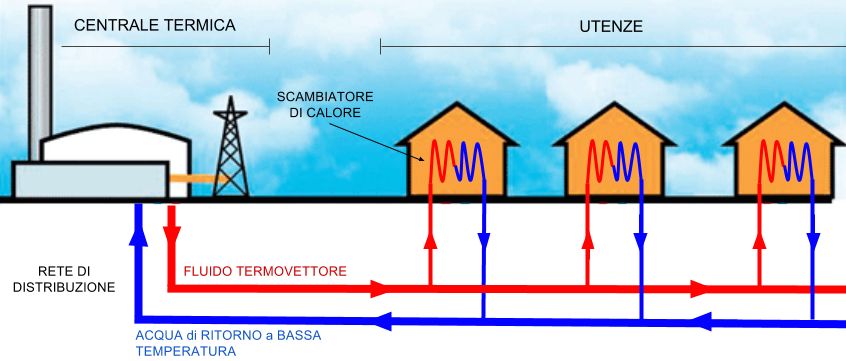
\includegraphics[width=1.0\textwidth]{figure/schema_impianto1}
\caption{Schema di un impianto di teleriscaldamento composto da: centrale di scambio, rete di distribuzione e sotto-centrali di scambio (scambiatori)}
\label{fig:schema1}
\end{center}
\end{figure}

La centrale termica riscalda l'acqua che viene distribuita ai diversi edifici attraverso la rete di distribuzione con l'ausilio di pompe. Giunta allo scambiatore, l'acqua della rete trasferisce all'acqua dell'impianto di distribuzione interno dell'edificio, il calore necessario per riscaldare gli ambienti e per la produzione di acqua calda sanitaria. L'acqua, ormai raffreddata, ritorna in centrale per essere nuovamente riscaldata. 
%Il teleriscaldamento riesce ad essere economicamente conveniente a patto che si riesca a trovare un bacino di utenze concentrate in un'area relativamente ridotta. La traduzione inglese di teleriscaldamento "district heating" che letteralmente tradotta vuol dire "riscaldamento distrettuale", rende l'idea della concentrazione che l'utenza dovrebbe avere per far sì che questo metodo sia economicamente vantaggioso. \\
In seguito si analizzerà più approfonditamente ogni elemento dell'impianto.

\subsection{Centrale termica e di scambio}
Le centrali termiche, analizzate nell'elaborato, sfruttano il vapore geotermico non idoneo alla generazione di energia elettrica. Le centrali di scambio si occupano dello scambio di calore tra due diversi circuiti. La centrale termica può essere interpretata come una centrale di scambio in quanto non fa altro che estrarre dal vapore l'energia termica da scambiare con l'intero impianto di teleriscaldamento. Il vapore, dunque, arriva in centrale a circa $240 ^{\circ}C$ e cede la sua energia termica attraverso gruppi di scambio termico costituito da uno scambiatore vapore-acqua surriscaldata a circa $120 ^{\circ}C$ e da un desurriscaldatore di condensa acqua acqua. La portata del vapore è controllata attraverso  valvole a due vie di tipo NC, in funzione della temperatura  di uscita dell'acqua surriscaldata desiderata nel circuito primario. La condensa viene raccolta in un serbatoio atmosferico e reiniettata nel punto di raccolta gestito da ENEL con pompe centrifughe multistadio, in modo da mantenere e rinnovare la risorsa geotermica. L'acqua surriscaldata viene inviata attraverso una linea feeder ad una seconda centrale di scambio, posta nei pressi del centro abitativo, dove cede la sua energia termica attraverso gruppi di scambio termico costituiti da uno scambiatore acqua surriscaldata - acqua calda. La portata di acqua surriscaldata è controllata attraverso valvole a due vie di tipo NC, in funzione della temperatura in uscita dell'acqua calda nela rete di distribuzione. Questo ulteriore scambio permette di separare la linea dell'acqua surriscaldata  dai circuiti urbani, che sono più estesi, riducendo così la potenza dell'impianto di pompaggio, le perdite di calore e il costo della rete. Inoltre, l'utilizzo di acqua calda anziché surriscaldata nei centri urbani, aumenta il livello di sicurezza e riduce gli interventi di manutenzione dovuti alla maggiore complessità degli impianti di utenza ad acqua surriscaldata. La circolazione sia nel circuito primario che secondario sono garantite da elettropompe centrifughe ubicate nella stessa centrale di scambio [figura \ref{fig:schema2}].
Nel caso in cui la centrale termica si trovi nei pressi delle utenze sarà possibile omettere la seconda centrale di scambio ed effettuare direttamente uno scambio di calore da vapore ad acqua calda [figura \ref{fig:schema3}].

 \begin{figure}[!ht]
 \centering
 \subfigure[Schema di un impianto di teleriscaldamento con due centrali di scambio. Questa configurazione è utilizzata quando la centrale termica è distante dal centro abitativo.\label{fig:schema2}]
   {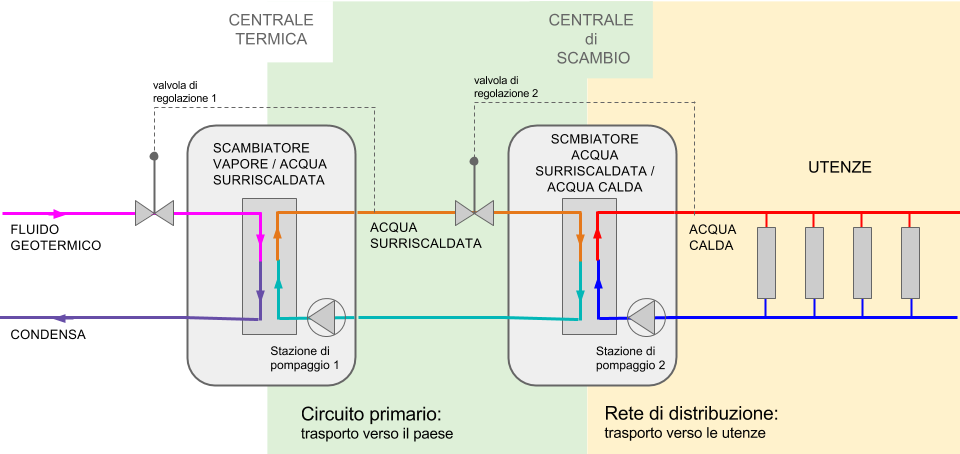
\includegraphics[width=12.5cm]{figure/schema_impianto2}}
 \hspace{5mm}
 \subfigure[Schema di un impianto di teleriscaldamento con singola centrale di scambio.\label{fig:schema3}]
   {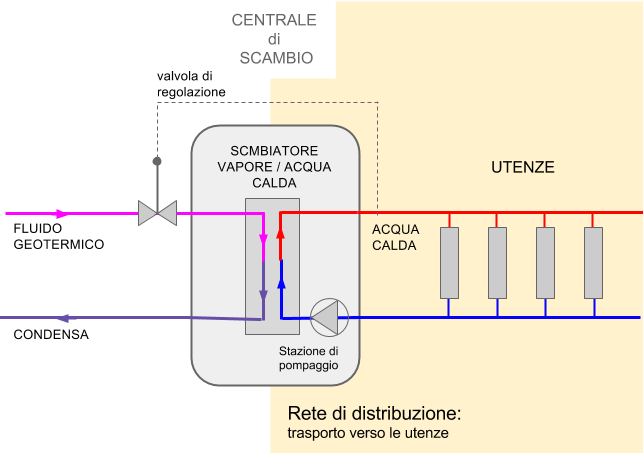
\includegraphics[width=8.5cm]{figure/schema_impianto3}}
 \caption{Possibili configurazioni di un impianto di teleriscaldamento alimentato da fonte geotermica}
 \end{figure}

%lavorano a regime variabile 
\subsection{Stazioni di pompaggio}
Le stazioni di pompaggio si occupano del trasporto dell'acqua verso le sotto-centrali di scambio delle utenze.
 
I parametri di maggiore rilevanza che contraddistinguono le pompe sono la portata e la prevalenza.\\
\textbf{Portata:} La portata della pompa è il volume d'acqua, misurato in litri o metri cubi, che viene mosso dalla pompa nell'unità di tempo (generalmente secondi o minuti). La portata si misura pertanto in litri al secondo ($l/sec$), litri al minuto ($l/min$), metri cubi all'ora ($m^3/h$), ecc...\\
\textbf{Prevalenza:} La prevalenza della pompa rappresenta l'incremento di energia acquisito da 1 $kg$ di liquido fra la sezione di entrata e quella di uscita della pompa stessa; generalmente si indica con $H$ e si misura in $J/kg$ oppure in metri ($m$) di liquido trasportato. Molto più comodo è parlare non di prevalenza bensì di prevalenza manometrica, indicata con $Hm$ e misurata in $m \ C.A.$ (metri di colonna d'acqua).

Le pompe solitamente usate sono pompe centrifughe, la cui curva caratteristica, in funzione della portata e della prevalenza, rimane abbastanza piatta per gran parte del range di portata. 
Il punto di funzionamento, ovvero la portata e la prevalenza emessa delle pompe, dipende dalla resistenza offerta dalla rete dell'impianto. 
Le stazioni di pompaggio sono solitamente localizzate dentro la centrale di scambio ed hanno il compito assicurare un flusso di acqua tale da offrire ai complessi abitativi l'energia termica richiesta. Per di più, devono fornire alle utenze più sfavorite una differenza di pressione tale da garantire il passaggio di acqua all'interno dello scambiatore d'utenza. 
Quando la portata è elevata, le perdite di pressione nella rete aumentano e le pompe dovranno lavorare più duramente. La pressione sarà sempre sufficiente nelle nelle sotto-stazioni vicine alla centrale, ma se la capacità limite della pompa viene raggiunta, la pressione nelle parti distanti della rete  possono decadere e gli scambiatori di calore di quelle zone non potranno lavorare correttamente. I radiatori di queste utenze svantaggiate saranno freddi.

Come già citato, le pompe sono i principali elementi responsabili dei consumi di un impianto di teleriscaldamento perciò è necessario introdurre delle regolazioni che limitino il più possibile gli sprechi di energia di pompaggio ma allo stesso tempo si deve far si che in tutte le utenze sia garantita una differenza di pressione che permetta il corretto funzionamento degli scambiatori. 


%Le pompe solitamente usate sono pompe centrifughe, la cui curva caratteristica in funzione della portata e della prevalenza rimane abbastanza piatta per gran parte del range di portata. In base alla resistenza che offerta dalla rete la pompa lavorerà su uno specifico punto di funzionamento, il quale a sua volta è responsabile  
%Risulta dunque fondamentale avere una regolazione per evitare lo spreco di energia di pompaggio. 
%Nel caso vi siano due stazioni di pompaggio, e quindi due centrali di scambio, possiamo regolare  sia le pompe che alimentano il circuito primario che quelle della rete di distribuzione. Le pompe che alimentano il circuito primario sono regolate in base al grado di laminazione della valvola nella seconda centrale di scambio, la quale garantisce che la temperatura dell'acqua in mandata nella rete di distribuzione rimanga costante al valore desiderato.  Più che la valvola risulta laminata più che aumenta la resistenza idraulica sul circuito primario, portando, di conseguenza, ad una riduzione della portata e ad un aumento della prevalenza nel circuito. La regolazione delle pompe che alimentano la rete di distribuzione dipendono dalle diverse esigenze di utilizzo idrico durante l'arco della giornata. 
%In impianti dove è presente una sola centrale di scambio l'unica taratura verrà effettuata sulla velocità delle pompe che inviano acqua nella rete di distribuzione affinché tutte le utenze possano usufruire della portata necessaria per soddisfare il proprio fabbisogno termico.
%Dal momento che gli elementi che dovrebbero fornire informazioni sulla regolazione della velocità delle pompe si  trovano in luoghi diversi e distanti rispetto al posizionamento delle stazioni di pompaggio, sono adottati i seguenti metodi di regolazione della potenza delle pompe:
%\begin{enumerate}
%\item Regolazione a pressione costante
%\item Regolazione a differenza di temperatura costante
%\end{enumerate}
%
%%\subsection{Regolazione a pressione costante}
%Nel seguente tipo di regolazione viene misurata la pressione in mandata del circuito primario e la pressione sul ritorno dello stesso circuito.  Laminando la valvola di regolazione otteniamo una dispersione di energia sulla valvola stessa tanto più grande tanto è maggiore il suo livello di chiusura. La laminazione comporta un aumento della resistenza idraulica e lo spostamento del punto di funzionamento della pompa. Il fenomeno è descritto in figura \ref{fig:dP}.
%
%Con i sistemi di regolazione  a pressione costante la pompa in servizio viene pilotata a velocità variabile mediante un convertitore di frequenza (Inverter). La velocità di rotazione dell'elettropompa viene adeguata istantaneamente in base alla pressione differenziale di erogazione impostata. Il punto di funzionamento perciò si posizionerà sulla retta orizzontale che definisce la variazione di prevalenza $\Delta H$ di set-point, rendendo necessario far lavorare la pompa a giri ridotti riducendo i consumi.
%
%$P_1$, il punto di funzionamento con valvola tutta aperta con portata $G_1$ e prevalenza $H_1$. Chiudendo la regolazione la resistenza idraulica aumenta facendo alzare più velocemente la curva caratteristica dell'impianto primario spostando il punto di funzionamento in $P_2$ con portata  $G_2$ e prevalenza $H_2$. 
%
%
%\subsection{Regolazione a differenza di temperatura costante}

\subsection{Rete di distribuzione}
La rete di distribuzione è la linea che trasporta acqua calda alle utenze verso le sotto-centrali di scambio. La rete è composta da tubazioni interrate che  devono  essere adeguatamente isolate  in  modo  da  evitare  che  la temperatura  del fluido termovettore si abbassi troppo lungo il tragitto. 
Il  lemma  inglese  stesso,  district  heating,  indica  l'importanza  che  ha  il  fattore  di localizzazione  di un sistema  di  teleriscaldamento, infatti,  l'area  teleriscaldabile  deve  essere  preferibilmente  un distretto  urbano,  cioè  un'area  ad  alta  densità  abitativa,  dove  le  costruzioni  sono abbastanza concentrate.
Aree  con  edifici  troppo  isolati  tra  loro  non  sono  infatti  convenienti  da  teleriscaldare, poiché
la rete di tubazioni si estenderebbe troppo e aumenterebbero le dispersioni di calore.
I terminali della rete di distribuzione sono le sotto-centrali di scambio (scambiatori). Da un punto di vista idraulico gli scambiatori di utenza vengono visti come una resistenza variabile che definiscono la caratteristica dell'impianto. 
Se nella rete di distribuzione non vi sono regolazioni sulla portata in ingresso alla sotto-centrale di scambio delle utenze, tutta la portata circolerà nei primi scambiatori e per alimentare gli ultimi si dovrà pompare un maggior quantitativo di acqua. Inoltre, avendo le prime utenze un surplus in portata, il calore disponibile sarà di gran lunga superiore a quello necessario. 
%perciò si scambierà solo una piccola parte di energia con la conseguenza che le temperature di ritorno saranno più alte.
L'introduzione di elementi che regolano la portata in ingresso allo scambiatore in base calore necessario all'utenza, risultano fondamentali per l'ottimizzazione di un impianto. 

% Centraline d'utenza ben configurate dovrebbero assicurare:
%\begin{itemize}
%\item limite sulla portata allo stretto indispensabile
%\item riduzione delle temperature di ritorno dello scambiatore
%\item aiutare l'utilizzatore a fare efficienza ovvero ridurre i consumi
%\end{itemize} 
%Questi elementi di regolazione sono inoltre un luogo dove si possono rilevare molte informazioni utili per l'ottimizzazione del circuito ad esempio le condizioni di arrivo dei fluidi nei punti estremi della rete non facilmente prevedibili istante per istante in quanto dipendono dalle richieste del momento di tutte le utenze precedenti .
%Dalle centraline si possono inoltre fare analisi di predittiva sullo stato di funzionamento degli scambiatori con segnalazione di anomalie che portano ad interventi programmati invece che in accidentale .

%\section{Analisi degli elementi critici}
%L'alimentazione da fonte geotermica di un impianto di teleriscaldamento garantisce un notevole risparmio in termini di gestione dell'impianto in quanto la potenza termica a disposizione risulta quasi a costo zero. Ne consegue che i principali consumi siano dovuti all' energia elettrica necessaria per il pompaggio delle acque di circolazione. Questa caratteristica,  che contraddistingue questi impianti di teleriscaldamento garantisce agli utenti dei costi di gran lunga inferiore rispetto agli impianti che devono produrre calore autonomamente. 
%Le stazioni di pompaggio lavorano a regime variabile e per una ottimizzazione del sistema, bisogna far si che le pompe sprechino minor energia possibile. 
%L'allacciamento di molte nuove utenze alle reti già esistenti e quindi la relativa  espansione della rete di distribuzione del calore, la mancanza di regolazioni nella rete distributiva e la non ottimizzazione della velocità delle pompe ha reso gli impianti inefficienti, con un conseguente aumento dei costi in bolletta. Questa situazione è ancor più amplificata nella stagione estiva in quanto le utenze utilizzano l'impianto di teleriscaldamento soltanto per la produzione di acqua calda sanitaria. L'energia di pompaggio per garantire all'utenza più critica la quantità di acqua necessaria al suo fabbisogno, supera di gran lunga l'energia realmente consumata dalle utenze. Questo ha portato all'inevitabile conseguenza della chiusura degli impianti in quel periodo.
%Gli elementi della rete che influiscono su questo fenomeno sono:
%\begin{enumerate}
%\item Stazioni di pompaggio
%\item Rete di distribuzione
%\end{enumerate}

\section{Effetti delle temperature di esercizio in un impianto di teleriscaldamento}
Le temperature di esercizio in una rete di teleriscaldamento  influenzano: la quantità di calore fornito alla rete, le perdite di calore e l'energia di pompaggio per il trasporto dell'acqua.

Vi sono due differenti temperature da tenere in considerazione: la temperatura di mandata e la temperatura di ritorno alla centrale di scambio. La prima è quella alla quale viene inviata l'acqua verso le utenze. Questa temperatura è prodotta dalla centrale termica. La seconda, è quella di ritorno dagli scambiatori di utenza, quindi a temperatura più bassa. La temperatura di ritorno non è un parametro che può essere settato ad un certo valore noto, ma è il risultato di uno scambio di calore che avviene nello scambiatore delle abitazioni, quindi è influenzata principalmente dalle utenze stesse.
Gli effetti che comportano le variazioni di queste due temperature sono descritti in seguito da un punto di vista generale. 

\subsection{Influenze sulla capacità termica in mandata}
Nelle reti di teleriscaldamento ci sono due parametri che controllano la potenza termica inviata alle utenze. L'equazione in seguito mostra come la suddetta potenza $P$ in arrivo alla sotto-centrale di scambio dipende dalla differenza di temperatura tra acqua in ingresso e quella in uscita dallo scambiatore $\Delta T$, dalla portata $\dot{m}$ e dalla capacità termica $C_p$ del fluido termovettore.
\begin{equation}
P = \dot{m} \ C_p \ \Delta T 
\label{eq:Potenza}
\end{equation} 

\begin{equation}
\Delta T = T_{mandata} - T_{ritorno}
\label{eq:dT}
\end{equation}

$C_p$ è una proprietà che dipende dal fluido per questo non viene considerata come un parametro che può influenzare la variazione di potenza inviata. Soltanto la portata e la differenza di temperatura   possono essere usate a questo scopo. La temperatura di ritorno $T_{ritorno}$ non è determinata dalla centrale di produzione. Soltanto la temperatura in mandata $T_{mandata}$ e la portata possono essere modificate dal gestore dell'impianto.
Questi due parametri sono gli strumenti che la centrale possiede per fornire la giusta quantità di calore in ogni momento.
% Si può variare anche soltanto un paramentro alla volta...

Dall'equazione \ref{eq:Potenza} è possibile notare come la potenza inviata alla rete di distribuzione sia proporzionale alla differenza di temperatura del fluido. Ogni volta che diminuisce la temperatura di ritorno oppure cresce la temperatura di mandata si ha una crescita della potenza totale trasportata a parità di portata.

Un sistema di teleriscaldamento efficiente ha due caratteristiche: una temperatura in mandata bassa e una differenza di temperatura tra mandata e ritorno alta. Una temperatura in mandata bassa fa diminuire le perdite di calore durante il trasporto, mentre, un $\Delta T$ alto comporta una riduzione della portata se si vuole mantenere invariata la potenza termica inviata.

Dal momento che la temperatura di ritorno non è un parametro che può essere deciso a priori, il maggiore sforzo per aumentare l'efficienza delle reti di teleriscaldamento, si ottiene regolando e ottimizzando le sotto-stazioni di scambio delle utenze, così da ottenere sempre la più bassa temperatura di ritorno. L'obiettivo si raggiunge fornendo alle abitazioni il suo reale fabbisogno di calore ed individuando i malfunzionamenti che riducono l'efficienza degli scambiatori. 
%Return temperatures depends mostly on the house heating systems. The old systems are designed to work with supply temperatures of 80 oC and return of 60 oC, whereas the modern ones use 60/45 oC
\subsection{Influenza sull'energia di pompaggio}
L'energia di pompaggio è l'energia necessaria al trasporto dell'acqua calda dalla centrale termica verso le utenze e per riportarla indietro alla centrale stessa. La perdita di pressione della rete deve essere misurata lontano dalla stazione di pompaggio e se la differenza di pressione tra mandata e ritorno non è sufficientemente elevata si ordina alla pompa di dare più pressione.

Queste pompe devono inviare una prevalenza tale da far fronte alle perdite di carico che si hanno lungo la rete e devono garantire una differenza di pressione sufficiente al corretto funzionamento degli scambiatori. Le perdite sono dovute principalmente alla frizione offerta dalle tubazioni al passaggio di acqua. Questa sorta di attrito non ha una relazione lineare con la portata, ma è approssimativamente proporzionale alla terza potenza della portata. Ciò implica che una diminuzione del flusso ha un grande impatto sulla riduzione delle perdite di pressione.

Dando uno sguardo all'equazione \ref{eq:Potenza} possiamo notare che a parità di potenza inviata alla rete, un aumento della differenza di temperatura comporta una diminuzione della portata del fluido e dunque, una diminuzione dei costi di pompaggio.

%Concludendo, l'aumento della differenza di temperatura ha un impatto notevole sul risparmio di energia elettrica.


\subsection{Influenza sulle perdite di calore}
Le perdite di calore in una rete di teleriscaldamento sono proporzionali alla differenza di temperatura tra l'ambiente e l'acqua nelle tubazioni. Dal momento che la temperatura ambiente è una variabile non decisionale, le perdite di calore dipendono dalla temperatura in mandata, da quella di ritorno e dalla portata. Le perdite di calore non sono un elemento da sottovalutare, infatti, in media il calore disperso in una rete è più alto del $10\%$ dell'energia fornita. Pertanto è importante tenere in considerazione questo tipo di perdite quando vogliamo determinare le temperature di esercizio ottimali di un impianto teleriscaldato.

Si potrebbe pensare che ridurre il più possibile la temperatura in mandata eliminerebbe il problema delle perdite di calore nei tubi. Se da una parte una temperatura in mandata molto bassa risolverebbe il problema, dall'altra si avrebbe che le pompe dovrebbero inviare un flusso di acqua molto maggiore per raggiungere la stessa potenza termica desiderata. Ai fini del problema, si dovrebbero trovare le temperature e le portate  della rete che minimizzano l'energia elettrica necessaria alle pompe per la circolazione dell'acqua sommata all'energia termica persa. Ogni termine della somma dovrà essere pesato 
in funzione dei differenti costi tra energia elettrica e produzione di calore.
Un altro vincolo importante sulla temperatura in mandata è che questa non potrà essere inferiore alla temperatura di funzionamento dei radiatori.  

\section{Effetti degli utenti sulla rete e tecnologie in uso per aumentare l'efficienza delle utenze}
Gli utenti svolgono un ruolo importante nell'ottimizzazione di un impianto di teleriscaldamento. Al fine di minimizzare l'energia elettrica consumata dalle stazioni di pompaggio, la differenza di temperatura tra mandata e ritorno deve essere massimizzata. La temperatura di mandata è un parametro prodotto dalla centrale termica, ma non la temperatura di ritorno. Quest'ultima dipende principalmente dagli utenti. Una bassa temperatura di ritorno è possibile soltanto se l'impianto dell'utenza è progettato a dovere e funziona correttamente.
La rete di distribuzione, ovvero la rete di tubi tra la centrale termica e le sottostazioni di scambio delle utenze, deve fornire alle utenze la potenza necessaria al proprio fabbisogno, quindi il flusso di acqua dovrà essere settato in modo da raggiungere tale potenza in funzione della temperatura in mandata e quella di ritorno. Quando nel circuito dell'utenza non viene mantenuta un alta differenza di temperatura tra mandata e ritorno, più portata sarà richiesta nella rete di distribuzione per trasferire la stessa potenza termica,
%. Per questa ragione, quando l'utenza ritorna acqua ad alta temperatura, nella sottostazione dovrà essere fornito un flusso maggiore, 
comportando un aumento dell'energia di pompaggio.

La differenza di temperatura deve essere massimizzata al fine di lavorare con il minimo flusso di acqua richiesto. Questa considerazione è valida sia per la rete di distribuzione che per il circuito dell'utenza a causa di una stretta relazione tra i due. 
Quando c'è una diminuzione del $\Delta T$ nel lato utenze si avrà un aumento della temperatura di ritorno anche dal lato della rete di distribuzione. Per mantenere la stessa potenza, dobbiamo aumentare la portata e questo aumento di flusso da una parte aumenta la quantità di energia termica, dall'altra, la maggiore velocità del liquido fa raffreddare meno il fluido per unità di tempo. 

Nella rete di distribuzione il flusso di acqua è regolato in accordo al carico termico richiesto. Durante l'inverno, dove la domanda è più alta, il flusso di fluido termovettore sarà più alto rispetto all'estate. Un flusso variabile nella rete è la strada necessaria da percorrere per ottimizzare le spese di pompaggio.

Nel circuito delle utenze può essere fatta la stessa considerazione. Tre differenti soluzioni per regolare la portata in arrivo alle sotto-centrali di scambio delle utenze verranno analizzate in seguito, tenendo condo di quanto e come influenzano la rete.

\subsection{Regolazione con valvola a tre vie}
\label{subsec:3vie}
La prima soluzione che verrà descritta lavora con un flusso costante di acqua che arriva allo scambiatore d'utenza. Una valvola a tre vie regola la quantità di fluido termovettore che verrà usato dall'utenza. Vi è quindi un flusso variabile, ma la pressione rimane costante. Lo schema di funzionamento è illustrato in figura \ref{fig:3vie}.

% figura
\begin{figure}[!ht]
\centering
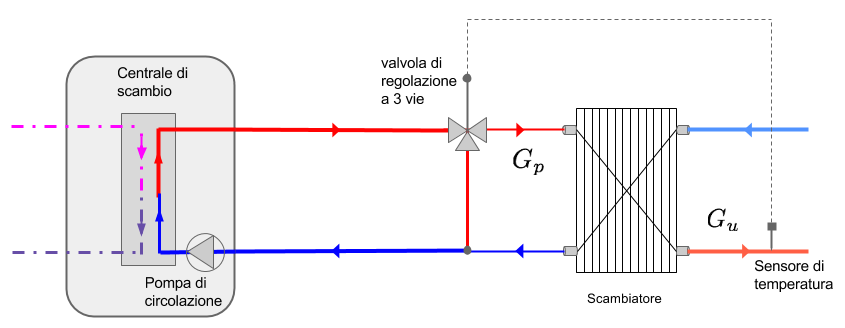
\includegraphics[width=0.9\textwidth]{figure/3vie}
\caption{Scema di funzionamento di una rete con valvola a tre vie}
\label{fig:3vie}

\end{figure}


La portata nella sotto-stazione dipende dalla quantità di calore necessario all'utenza. 

Quando questa ha bisogno di più energia, la temperatura sul ritorno del lato utenza inizia a diminuire a causa del consumo di calore. Il sensore sul ritorno rileva una temperatura più bassa sul circuito d'utenza e di conseguenza comunica alla valvola a tre vie di aumentare il flusso verso lo scambiatore in modo da avere un più alto trasferimento di calore dalla rete di distribuzione.
%Quando questa ha bisogno di più energia, la temperatura sul ritorno inizia a diminuire a causa del consumo di calore. La valvola a due vie sul primario  rileva una temperatura più bassa sulla rete di distribuzione e di conseguenza aumenta il flusso in modo da avere un più alto trasferimento di calore dal primario alla rete di distribuzione.
Nel sistema descritto, la valvola a tre vie decide in ogni momento quale è la portata necessaria in base al carico termico richiesto. Il resto dell'acqua è rimandato nella tubazione di ritorno attraverso il by-pass senza essere raffreddata. Conseguentemente, la temperatura di ritorno sarà più alta tanto più acqua è deviata. Più alta è la temperatura sul ritorno dell'utenza     più flusso di acqua sarà necessario per spedire la stessa potenza. In questo sistema la pompa sulla rete di distribuzione lavora sempre a massimo carico, senza dipendere dalla domanda di calore. Conseguentemente la vita delle pompe sarà più breve e le spese di pompaggio saranno alte.

\subsection{Regolazione con valvola di laminazione}
\label{subsec:2vie}
In questo caso, il flusso di acqua non è costante. Una valvola di laminazione (a due vie) regola la portata in base alla necessità di calore delle utenze. 
Come nel caso precedente, quando il sensore rileva una temperatura troppo bassa dell'acqua di ritorno del lato utenza, comunica alla valvola di laminazione di far passare più acqua. 
La suddetta valvola può essere vista come una resistenza che si oppone al passaggio del fluido. Maggiore è il grado di laminazione, maggiore è la resistenza offerta e minore risulterà la portata della rete di distribuzione. Considerando la pompa a regime costante, il grado di chiusura della valvola farà spostare il suo punto di lavoro lungo la curva caratteristica della pompa stessa, modificando così portata e pressione del fluido.
La portata in ingresso allo scambiatore dipenderà sempre da quanta potenza richiede l'abitazione e questo garantisce una temperatura di ritorno bassa. 
Il consumo di energia dipende in un certo senso dalla quantità di energia termica inviata. Essendo tale potenza variabile sarà possibile risparmiare più energia di pompaggio rispetto al primo caso con la valvola a tre vie dove la potenza inviata è costante. Lo schema di funzionamento è mostrato in figura \ref{fig:2vie}.

% figura
\begin{figure}[!ht]
\centering
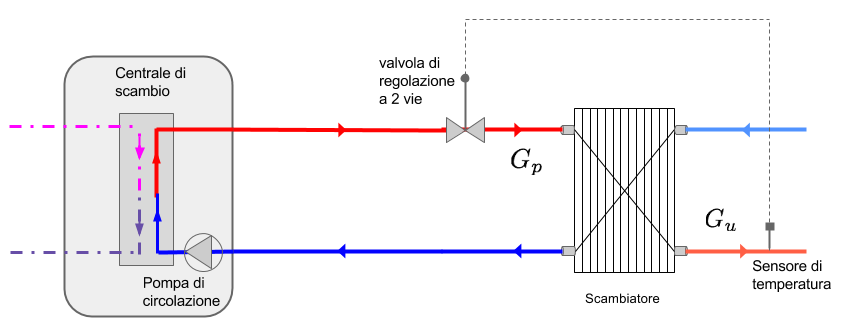
\includegraphics[width=0.9\textwidth]{figure/2vie}
\caption{Scema di funzionamento di una rete con valvola di laminazione(valvola a due vie)}
\label{fig:2vie}

\end{figure}

La rete di distribuzione diventa un sistema con portata e pressione variabile. Viene solitamente scelto dagli ingegneri in quanto ha bisogno di poca manutenzione, riduce i consumi di energia elettrica per il pompaggio e assicura una bassa temperatura di ritorno.

Sia nel primo che nel secondo caso il sensore di temperatura può essere messo sulla tubazione che porta l'acqua ai radiatori anziché su quella di ritorno. In questo modo si definisce un target di temperatura da mantenere. Questo set point dovrà essere impostato in base al tipo di impianto.

\subsection{Regolazione con pompe a temperatura di ritorno costante}
Vengono utilizzate come in \ref{subsec:3vie}, delle valvole a tre vie per regolare il flusso agli scambiatori di utenza. In questo caso però, vi è la possibilità di far variare la velocità delle pompe al fine di ridurre il più possibile i consumi per il pompaggio di acqua.
La velocità viene regolata in modo da mantenere la temperatura dell'acqua di ritorno in centrale di scambio ad un valore costante. La temperatura è misurata da un sensore, successivamente viene confrontata con quella desiderata e viene valutato se modificare il numero di giri delle pompe. 
Quando un utenza richiede poca energia termica, la valvola devia gran parte del fluido caldo sulla condotta di ritorno, comportando un aumento della temperatura del liquido. Il sensore rileva questa variazione e comunica alla pompa di diminuire la velocità in quanto l'acqua di ritorno dalle utenze è troppo calda. Ciò implica che il fabbisogno di calore in quel momento è basso e quindi, stiamo inviando più energia di quanta realmente è necessaria. Se l'acqua di ritorno è più fredda del valore desiderato si aumenterà il numero di giri delle pompe. 

Modificando la velocità delle pompe si modifica sia la portata che la prevalenza della stessa e dunque anche i consumi di energia elettrica.

\subsection{Regolazione con pompe a pressione differenziale}
Ugualmente alla regolazione \ref{subsec:2vie}, si utilizza una valvola di laminazione per regolare il flusso di fluido all'utenza ma la principale differenza sta nell'introduzione di una pompa a velocità variabile, controllata in funzione della differenza di pressione tra la condotta di mandata e di ritorno dell'acqua, cosicché il consumo di elettricità per il pompaggio venga ridotto al massimo.
 La velocità della pompa è regolata al fine di mantenere una differenza di pressione costante prestabilita. Le variazioni di pressione nel circuito sono causate dal grado di chiusura della valvola a due vie. Quando la valvola si chiude, aumenta la pressione nel circuito e dei sensori percepiscono la variazione di pressione comunicando alle pompe di modificare il numero di giri in modo da riportare la pressione al valore desiderato. In figura \ref{fig:giri_variabili} sono analizzati i cambiamenti portati dai due miglioramenti.

% figure
\begin{figure}[!ht]
\centering
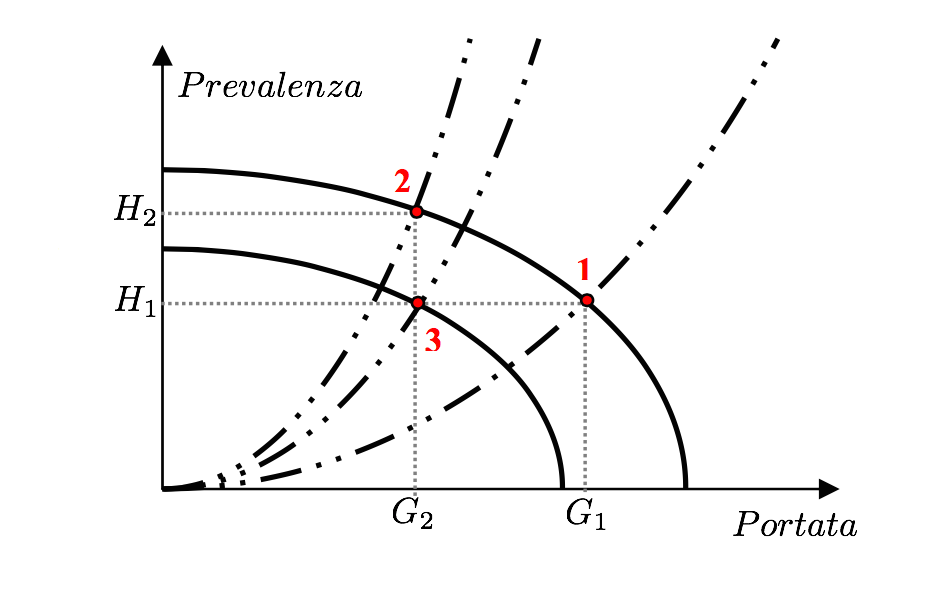
\includegraphics[width=0.8\textwidth]{figure/giri_variabili}
\caption{Cureve caratteristiche della pompa (linea continua) e curve di carico (linea tratteggiata)}
\label{fig:giri_variabili}
\end{figure}

Il punto 1 rappresenta un alta domanda di calore, quindi la portata sarà a sua volta alta. Se la domanda di calore decresce, la valvola di laminazione inizia a chiudersi facendo aumentare la resistenza del circuito e quindi la curva caratteristica della rete cresce più rapidamente. Il punto si lavoro si sposta quindi da 1 a 2. Il comportamento analizzato fino ad ora descrive il funzionamento della valvola di laminazione utilizzato anche nella regolazione a due vie della sezione \ref{subsec:2vie}. Se però viene introdotta una pompa a pressione differenziale costante, il punto di funzionamento da 1 verrà spostato a 3. Se la velocità della pompa è diminuita, la caratteristica della pompa verrà descritta da una nuova curva. Anche la curva di carico dell'impianto cambierà, avendo come risultato due curve che si intersecano nel punto 3.      

La regolazione della velocità delle pompe è uno dei modi migliori per diminuire al massimo i consumi delle pompe e ed è anche una delle migliori soluzioni per i gestori dell'impianto e per i consumatori. Con questo tipo di regolazione si dovrebbe ottenere il minore consumo di energia e la più alta differenza di temperatura possibile.

\section{Metodi per ridurre la temperatura di ritorno}  
% spostare la sezione in un altro capitolo

In una comune utenza la potenza termica necessaria al riscaldamento per raggiungere un certo set point dipende principalmente dalla temperatura esterna. Più all'esterno è freddo più saranno le perdite di calore dell'abitazione.

% ecc..



\chapter{Modelli Matematici}

\section{Scambiatore di calore}
\label{subsec:scambiatore_di_calore}
Gli scambiatori di calore sono  delle apparecchiature in cui si realizza lo scambio di energia termica tra due fluidi aventi temperature diverse. Negli impianti di teleriscaldamento solitamente vengono utilizzati scambiatori di calore a piastre, in cui due fluidi scorrono tra delle lastre metalliche piane, dotate di particolari rilievi per aumentare la superficie di scambio termico. In essi la trasmissione del calore avviene per convezione tra i fluidi e le rispettive superfici solide lambite e per conduzione attraverso la parete del tubo che li separa. Il tipo di contatto è di tipo indiretto in quanto non vi è miscelazione dei fluidi.
Il loro funzionamento è garantito soltanto dalla presenza di due fluidi a differente temperatura. La temperatura del corpo più caldo diminuisce, mentre la temperatura di quello più freddo aumenta. La progressiva riduzione della differenza di temperatura deve essere ricondotta a uno scambio di energia, scambio che continua finché esiste tale differenza termica, ovvero fino a quando non si raggiunge l'equilibrio termico. 

Le variabili in gioco sono elencate in seguito:
\begin{itemize}
\item[] $G_p$ = portata del circuito primario
\item[]$G_u$ = portata del circuito secondario (parte utenza)
\item[]$c_s$ = calore specifico dell'acqua
\item[]$T_i$ = Temperatura di ingresso scambiatore dalla parte del circuito primario (acqua calda)
\item[]$T_u$ = Temperatura in uscita dallo scambiatore dalla parte del circuito primario (acqua fredda)
\item[]$t_i$ = Temperatura di ingresso scambiatore dalla parte del circuito secondario (acqua fredda)
\item[]$t_u$ = Temperatura in uscita dallo scambiatore dalla parte del circuito secondario (acqua calda)
\end{itemize}

% CAMBIARE IMMAGINE
\begin{figure}[h]
\begin{center}
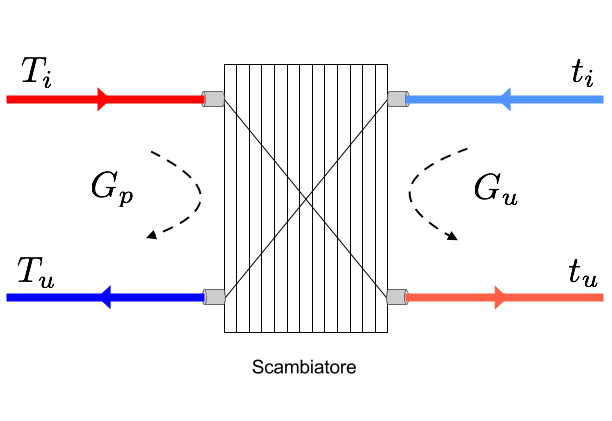
\includegraphics[width=0.65\textwidth]{figure/scambiatore} % Include the image placeholder.png
\caption{Schema di uno scambiatore d'utenza}
\label{fig:scamb}
\end{center}
\end{figure}

Applicando le equazioni di bilancio di massa e di energia al fluido caldo ed al fluido freddo, assumendo che non vi siano dispersioni di calore durante lo scambio, si ottengono le seguenti formule per il calcolo della potenza termica globale $\dot{Q}$. Nello studio degli scambiatori di calore è  utile riferirsi alla cosiddetta portata termica (oraria), $C$, data dal prodotto tra la portata massica ed il calore specifico:
\begin{equation}
C_p=G_p c_s  \ \ \ ; \ \ \ C_u=G_u c_s
\end{equation}
In tal caso le due equazioni di bilancio  possono scriversi nella seguente forma:
\begin{equation}
\dot{Q}=C_p(T_i - T_u) \ \ \ ; \ \ \ \dot{Q}=C_u(t_u - t_i)
\label{eq:scambiatore1}
\end{equation}
A queste due equazioni di bilancio energetico, si può associare una equazione di scambio termico; quest'ultima associa la potenza termica scambiata tra i due fluidi alle temperature di ingresso e/o di uscita, alle portate, al coefficiente di scambio termico globale ed all'area di scambio. Questa equazione deriva dal metodo della media logaritmica delle differenze di temperatura (o MLDT) dove  la potenza termica scambiata tra i due fluidi viene legata alla differenza di temperatura tra il fluido caldo ed il fluido freddo dalla seguente relazione:
\begin{equation}
\dot{Q}=\alpha S \Delta T_{ml} \\
\end{equation}
\begin{equation}
 \Delta T_{ml} = \frac{(\Delta T_1)-(\Delta T_2)}{log\left( \frac{\Delta T_1}{\Delta T_2} \right)} \\
 \label{eq:scambiatore2}
 \end{equation}
 \begin{center}
 Se scambiatore in corrente : $ \Delta T_1 = T_i - t_i $  \ \ ; \ \ $ \Delta T_2 = T_u - t_u $  \\
 
 Se scambiatore in controcorrente : $ \Delta T_1 = T_i - t_u $  \ \ ; \ \ $ \Delta T_2 = T_u - t_i $ 
\end{center}
dove $S$ \`e  la superficie attraverso cui avviene lo scambio ed $\alpha$ \`e  il cosiddetto coefficiente di scambio termico globale o conduttanza termica unitaria. 

In figura \ref{fig:andamento} è  possibile vedere l'andamento delle temperature negli scambiatori in corrente (a) e in controcorrente (b).
Nel caso dello scambiatore equicorrente si ha una forte differenza di temperatura all'ingresso e una differenza  minima  all'uscita.  Nel  caso  dello  scambiatore in controcorrente  la  differenza  è invece più costante e il fluido freddo può uscire dallo scambiatore a temperatura maggiore di  quella  dell'uscita del fluido  caldo. 
Termodinamicamente quindi  questa  configurazione  è superiore, per  la  minore  caduta di temperatura dell'energia termica.

\begin{figure}[h]
\begin{center}
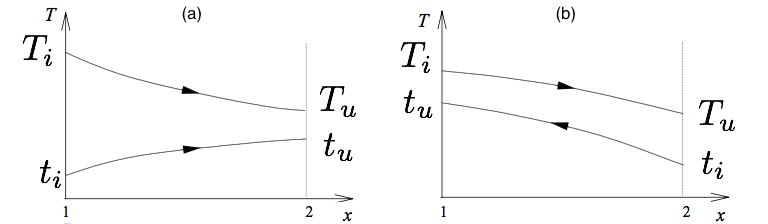
\includegraphics[width=0.95\textwidth]{figure/grafico_scambiatore} % Include the image placeholder.png
\caption{Andamento delle temperature negli scambiatori }
\label{fig:andamento}
\end{center}
\end{figure}

\section{Radiatori}
\label{subsec:radiatori}
I radiatori sono gli elementi all'interno dell'utenza che trasferiscono calore all'ambiente per scaldarlo. 
La potenza emessa da un corpo scaldante dipende dalla sua temperatura media tra il fluido caldo in ingresso al radiatore e quello freddo in uscita ($t_u$ e $t_i$ rispettivamente) dalla seguente relazione:
\begin{equation}
\dot{Q}_{ri}= K_m(\frac{t_u + t_i}{2} - \Theta_{i})^n
\label{eq:potenza_radiatori}
\end{equation}
con $K_m$ e $n$ coefficienti costanti che dipendono dal tipo di radiatore utilizzato e $\Theta_i$ la temperatura ambiente della casa. 
Il funzionamento di questi elementi di riscaldamento è garantito da una pompa di circolazione solitamente a velocità fissa che permette la circolazione di acqua calda all'interno dell'abitazione. 

Un'analisi importante riguarda il comportamento dei radiatori in termini di calore scambiato al variare della portata. Considerando la temperatura in mandata ai radiatori costante, la temperatura di ritorno dipende  dalla velocità con cui scorre il fluido nei radiatori, quindi la portata è uno dei fattori determinanti della temperatura media e quindi della potenza emessa dai radiatori. Maggiore è la portata minore sarà il tempo per scambiare calore, avendo così una temperatura di ritorno e una conseguente temperatura media più alta e viceversa. Si può fare riferimento all'equazione \ref{eq:Potenza}, valida anche per i radiatori, per notare come la portata sia direttamente proporzionale alla potenza termica scambiata. 

E' possibile ottenere  le stesse potenze termiche con due portate diverse facendo variare la differenza di temperatura tra fluido caldo e freddo, e di conseguenza alzando o abbassando le temperature di mandata dei radiatori [figura \ref{fig:portata}]. 
%Diminuendo la portata il radiatore scambia di più  e ciò  comporta una riduzione dell'acqua di ritorno dal radiatore. Se però  la temperatura in mandata rimane la stessa avremo una potenza scambiata dal radiatore minore in quanto si \`e  abbassata la temperatura media del fluido all'interno del radiatore (figura \ref{fig:portata}).

\begin{figure}[h]
\begin{center}
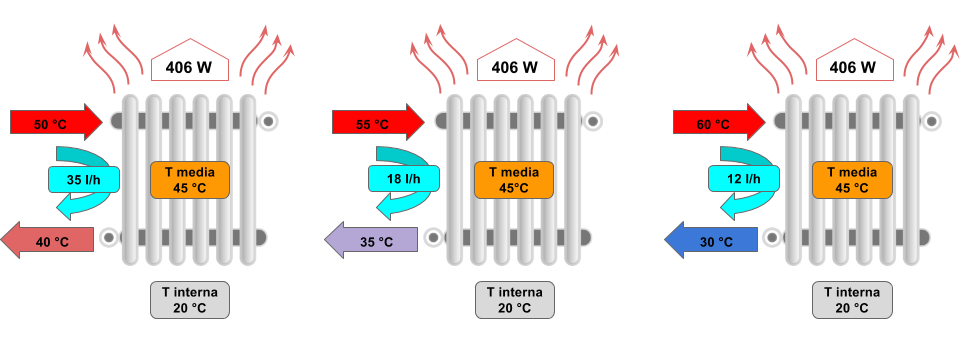
\includegraphics[width=0.95\textwidth]{figure/portata} % Include the image placeholder.png
\caption{Mantenimento delle potenze scambiate dal radiatore costante variando la temperatura di mandata e la portata.}
\label{fig:portata}
\end{center}
\end{figure}

Dal momento che, come detto in precedenza, le pompe solitamente lavorano a velocità costante, se vogliamo ottenere una potenza maggiore l'unica opzione possibile è quella di aumentare la temperatura in mandata in modo da far aumentare la temperatura media [figura \ref{fig:portata2}].

\begin{figure}[h]
\begin{center}
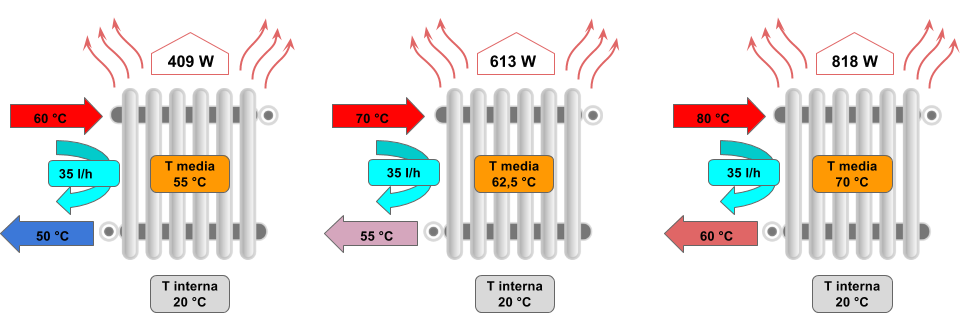
\includegraphics[width=0.95\textwidth]{figure/portata2} % Include the image placeholder.png
\caption{Variazione delle potenze scambiate radiatore variando la temperatura di mandata variabile e mantenendo la portata costante.}
\label{fig:portata2}
\end{center}
\end{figure}

\section{Dinamica dell'utenza}
\label{sec:dinamicautenza}
In seguito è descritto il modello utilizzato in simulazione per modellare gli scambi termici all'interno di un edificio. 
Il trasferimento di calore tra due mezzi può avvenire per conduzione o convezione ed è proporzionale alla differenza di temperatura tra i due mezzi coinvolti. Il trasferimento di calore per conduzione e convezione può quindi essere modellato utilizzando una resistenza termica,
\begin{equation}
\dot{Q} = \frac{1}{R} (T_1-T_2)
\label{eq:q1}
\end{equation}
dove $T_1$ e $T_2$ sono le temperature di ogni mezzo coinvolto nello scambio di calore mentre $R$ è la resistenza opposta al trasferimento l'energia termica.

L'altro aspetto importante da tenere in considerazione è la capacità termica, la quale descrive quanto un materiale  è in grado di accumulare calore. Nella seguente equazione è descritta la relazione che lega la capacità termica $C$ con il calore trasferito $\dot{Q}$ e la temperatura $T$.
\begin{equation}
\dot{Q} = C(T) \frac{dT}{dt} \approxeq C \frac{dT}{dt}
\label{eq:q2}
\end{equation}
Dal momento che l'intervallo di temperature in cui opera la casa è piccolo, possiamo quindi assumere la capacità termica come costante.

La termodinamica dell'utenza è modellata su una grande stanza circondata da pareti ed i flussi termici sono schematizzati in figura \ref{fig:scambio}. Gli scambi di calore che possono avvenire sono: scambio di calore tra i radiatori e l'aria della stanza, scambio di calore tra l'aria della stanza e le pareti, scambio di calore tra le pareti e l'esterno.

\begin{figure}[h]
\begin{center}
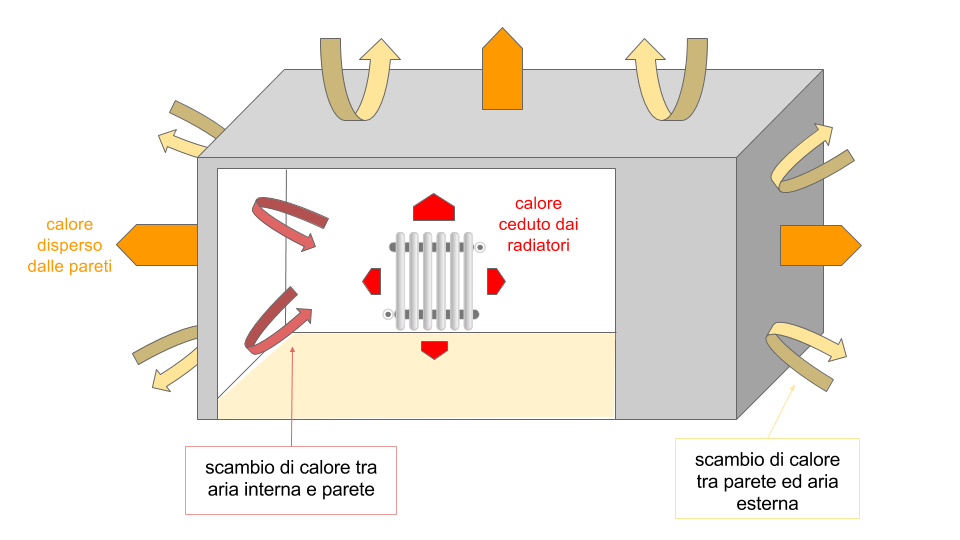
\includegraphics[width=1.05\textwidth]{figure/scambio_casa}
\caption{Scambi di calore di un abitazione generica}
\label{fig:scambio}
\end{center}
\end{figure}

Le grandezze che verranno usate nel modello da questo punto in avanti sono le seguenti:
\begin{itemize}
\item[] $\dot{Q}_{ri}$ = calore fornito dai radiatori
\item[]$C_i$ = capacità termica dell'aria all'interno dell'abitazione
\item[]$C_p$ = Capacità termica delle pareti
\item[]$R_{ip}$ = Resistenza termica tra l'aria interna alla casa e la parete
\item[]$R_{pe}$ = Resistenza termica tra la parete le l'aria all'esterno della casa
\item[]$R_{conv,i}$ = Resistenza termica per convezione   parete interna della casa
\item[]$R_{conv,e}$ = Resistenza termica per convezione  parete esterna della casa
\item[]$R_{cond}$ = Resistenza termica per conduzione della parete della casa
\item[]$\Theta_{e}$ = Temperatura dell'aria all'esterno della casa
\item[]$\Theta_i$ = Temperatura dell'aria all'interno dalla casa
\item[]$\Theta_p$ = Temperatura della superficie della parete all'interno dalla casa 
\item[]$A$ = Superficie di scambio delle pareti
\end{itemize}


A causa delle analogie tra le equazioni \ref{eq:q1} e \ref{eq:q2} con resistenze e capacità elettriche, possiamo modellare la termodinamica dell'abitazione come una rete elettrica, costituita da resistenze e condensatori, con le temperature equivalenti alle tensioni e il flusso di calore equivalente al flusso di cariche elettriche, ovvero alla corrente. Il circuito elettrico equivalente degli scambi di calore è mostrato in figura \ref{fig:RC}.

\begin{figure}[h]
\begin{center}
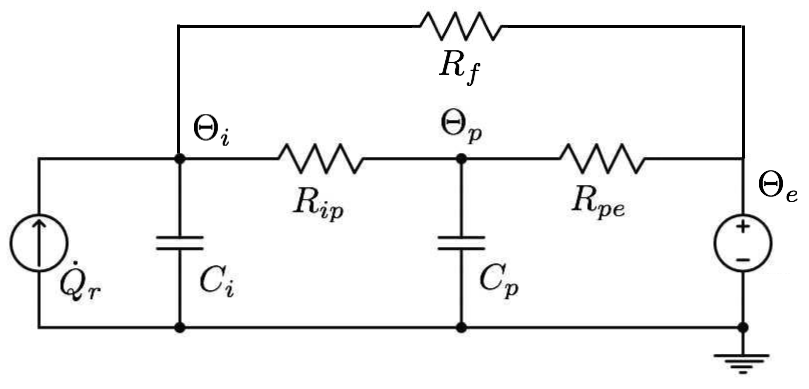
\includegraphics[width=0.75\textwidth]{figure/schema_trasf_calore}
\caption{Circuito equivalente RC per gli scambi di calore}
\label{fig:RC}
\end{center}
\end{figure}
 
Vediamo adesso in dettaglio come viene considerato lo scambio tra aria pareti ed esterno. L'aria interna che precedentemente ha ricevuto calore dai radiatori cede calore alla superficie interna delle pareti per convezione secondo la legge:
\begin{equation}
\dot{Q} = A \frac{(\Theta_i - \Theta_p)}{R_{ip}} 
\end{equation} 
Dal momento che la temperatura delle pareti a cui facciamo riferimento è quella della superficie interna dell'edificio la resistenza termica sarà data soltanto dalla resistenza termica per convezione, ovvero:
\begin{center}
$R_{ip} = R_{conv,i}$
\end{center}

Lo scambio tra la parete e l'ambiente esterno è dato dalla differenza di temperatura tra la parete interna e l'aria  esterna, considerando come resistenza termica la resistenza conduttiva $R_{cond}$ degli strati della parete e la resistenza convettiva sulla superficie esterna $R_{conv,e}$ per cui:
\begin{equation}
\dot{Q} = A \frac{(\Theta_p - \Theta_e)}{R_{pe}} 
%R_{conv,e} = \frac{1}{h_{conv,e}}
\end{equation} 
\begin{center}
$R_{pe} = R_{cond} + R_{conv_e}$
\end{center}

Il modello può essere formulato come un modello condensato a due stati di temperatura. La temperatura dell'aria all'interno della casa $\Theta_i$ e la temperatura delle pareti $\Theta_p$.

Riassumendo, l'aria, riscaldata dai radiatori a temperatura $\Theta_i$, scambia calore con la superficie interna delle pareti che si troverà a temperatura $\Theta_p$. In base alla superficie di scambio, la differenza di temperatura tra i due mezzi e la resistenza termica $R_{ip}$ tra aria e pareti, si otterrà un certo scambio termico verso di esse. L'energia scambiata viene accumulata dalla parete che funziona come un condensatore di capacità $C_p$. Parte dell'energia totale delle pareti invece viene ceduta all'esterno. Il calore ceduto dipenderà dalla superficie di scambio, dalla differenza di temperatura tra la parete interna e l'aria all'esterno dell'edificio, e la resistenza termica $R_{pe}$ che offre la parete con l'aria esterna.  Un equivalente elettrico del modello della parete è visibile in figura \ref{fig:RC_parete}.
Quando la potenza scambiata dall'aria alla parete  interna è maggiore di quella dispersa all'esterno si avrà un aumento della temperatura delle pareti stesse.

Da notare è anche il fatto che la temperatura all'interno della parete non è uniforme. Infatti, se prendessimo una sezione di una parete, vedremmo che in base alla distanza dalla sua superficie interna la temperatura decresce come mostrato in figura \ref{fig:temp_parete}.  Nel modello scelto si considera come temperatura di riferimento della parete la temperature della superficie interna della stessa. La scelta è stata fatta solamente per comodità, infatti si sarebbe potuto tenere in considerazione la temperatura della superficie esterna anziché quella interna. In base al punto al quale si fa riferimento per la temperatura, sarà necessario impostare  i valori di $R_{ip}$ e $R_{pe}$ appropriatamente.   

 \begin{figure}[h]
 \centering
 \subfigure[Circuito equivalente RC di una parete.\label{fig:RC_parete}]
   {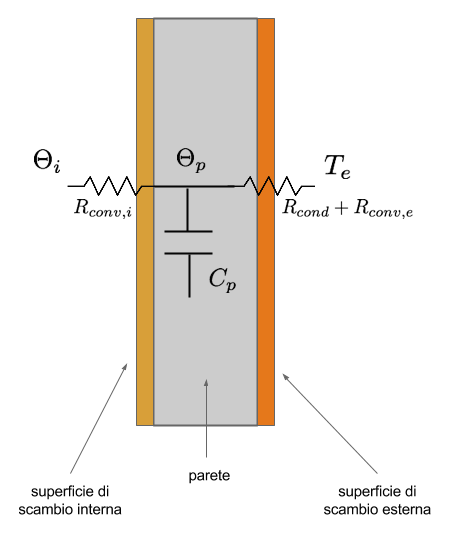
\includegraphics[width=4.6cm]{figure/RC_parete}}
 \hspace{5mm}
 \subfigure[Andamento della temperatura in una parete.\label{fig:temp_parete}]
   {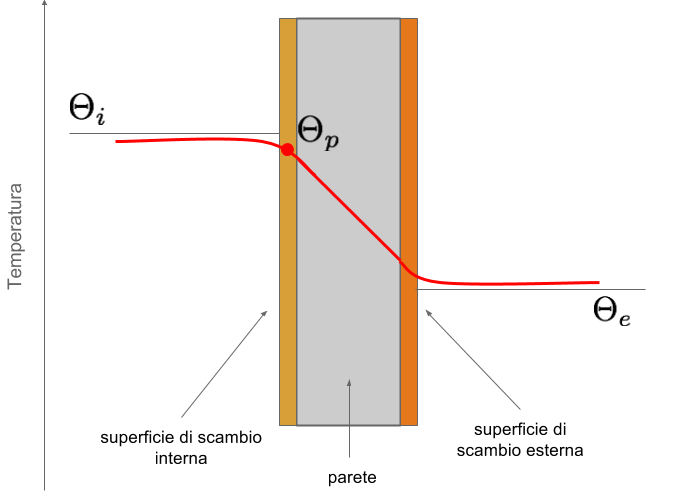
\includegraphics[width=6.2cm]{figure/temp_parete}}
 \caption{Schemi di funzionamento degli scambi termici in una parete di un'abitazione}
 \end{figure}
%\subsection{Utenza}
%Esiste ovviamente una formula matematica che consente un calcolo approssimativo del fabbisogno termico. Bisogna però tenere presente che è  un risultato indicativo e, appunto, approssimativo, poiché ci sono moltissime variabili che possono incidere sul reale fabbisogno dell'abitazione, alcune delle quali difficilmente quantificabili. 
%
%Il calcolo matematico fornisce il totale delle $Kcal$ necessarie a scaldare l'abitazione utilizzando come dati di partenza
%\begin{itemize}
%\item  il totale dei metri cubi da scaldare,
%\item    un coefficiente termico che indica le calorie necessarie per metro cubo e che può  oscillare tra un valore che va da 30 a 40 $\frac{Kcal}{m^3}$, a seconda delle condizioni termiche dell'abitazione.
%\end{itemize}
%Dunque il fabbisogno termico della casa può essere descritto dal prodotto tra il volume dell'utenza per il coefficiente termico scelto in base al tipo di abitazione.
%
%%Nei futuri calcoli considereremo  un appartamento di 100 $m^2$ con soffitti non pi\`u  alti di 3 $m$ e coefficiente termico di 30 $\frac{Kcal}{m^3}$. Il fabbisogno termico di risulter\`a  di circa 9000 $Kcal$ (10440 $W$).
%%
%%Questo valore ci da un indice di quanta energia i radiatori dovranno fornire alla casa per scaldarla.
%
%\subsubsection{Radiatori}

\section{Dinamica e interazioni tra scambiatore e utenza}
Per quanto riguarda la creazione di un simulatore dobbiamo trovare un modello matematico che descriva le interazioni che avvengono tra lo scambiatore di calore e l'utenza. In particolare è interessante sapere come si evolvono le temperature dell'acqua nello scambiatore e come varia la temperatura interna dell'abitazione al variare di alcuni parametri come la temperatura in ingresso allo scambiatore, la temperatura in mandata verso i radiatori, la portata, sia del lato della rete di distribuzione che del circuito dell'utenza e la temperatura esterna.
In figura \ref{fig:scamb_utenza} è rappresentato lo schema che descrive le interazioni e i parametri in gioco nel sistema composto dallo scambiatore di calore e dall'utenza. 

\begin{figure}[h]
\begin{center}
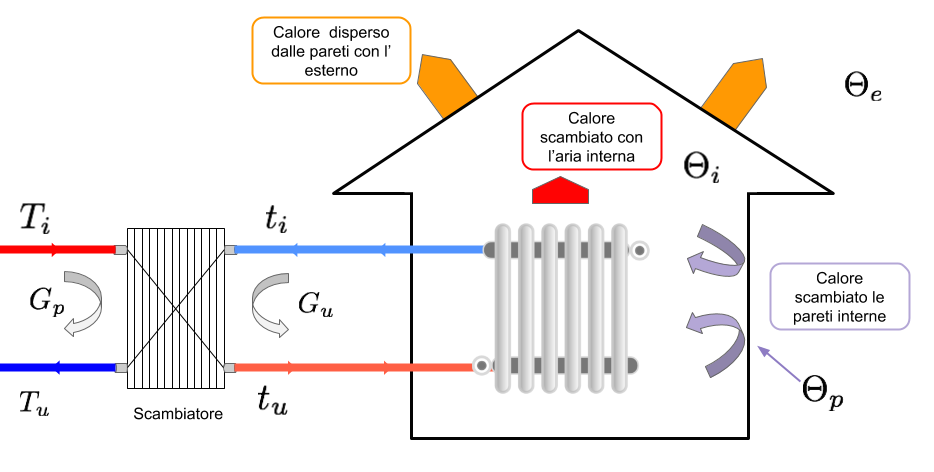
\includegraphics[width=0.9\textwidth]{figure/scamb_utenza} % Include the image placeholder.png
\caption{rappresentazione schematica sistema scambiatore e utenza}
\label{fig:scamb_utenza}
\end{center}
\end{figure}

%Come descritto nella sezione \ref{sec:dinamicautenza} 
Faremo riferimento ad un sistema dinamico con due variabili di stato: la temperatura interna all'utenza  $\Theta_i$  e dalla temperatura della superficie interna delle pareti  $\Theta_p$. Il sistema è  descritto  da due equazioni differenziali:
\begin{center}
$M_aC_a \dot{\Theta}_i = \dot{Q}_{ri} - \dot{Q}_{ip}$ 
\end{center}
\begin{center}
$M_pC_p \dot{\Theta}_p = \dot{Q}_{ip} - \dot{Q}_{pe}$
\end{center}
con $\dot{Q}_{ri}$ il\ calore scambiato tra i radiatori e l'aria interna alla casa, $\dot{Q}_{ip}$ il calore scambiato tra l'aria e la parete interna, $M_a$ la massa dell'aria all'interno dell'abitazione e $C_a$ la capacità termica dell'aria. Per la seconda equazione $ \dot{Q}_{pe}$ è il calore scambiato tra le pareti e l'ambiente esterno, $M_p$ la massa delle pareti e $C_p$ il calore specifico delle pareti.
Più in particolare:
\begin{equation}
K_m\left(\frac{t_u + t_i}{2} - \Theta_{i}\right)^n - \left(\frac{\Theta_{i} - \Theta_p}{R_{ip}}\right) = M_aC_a \dot{\Theta_i}
\end{equation}
\begin{equation}
\left(\frac{\Theta_{i} - \Theta_p}{R_{ip}}\right) - \left(\frac{\Theta_{p} - \Theta_e}{R_{pe}}\right) = M_pC_p \dot{\Theta_p}
\end{equation}



\`E possibile analizzare due differenti scenari:
\begin{itemize}
\item \textbf{Scambiatore senza regolazione di portata}: si tratta di avere uno scambiatore d'utenza senza alcun tipo di regolazione sulla portata. In questo caso non è possibile definire nessun set point di temperatura in mandata ai radiatori. Le variabili note sono $G_u, T_i, G_p$ mentre quelle incognite sono: $T_u, t_u, t_i$

\item \textbf{Scambiatore con regolazione di portata} si analizza uno scambiatore con regolazione in portata. Con questo tipo di configurazione vi è la possibilità di fissare la temperatura in mandata ai radiatori. Questa temperatura viene mantenuta costante agendo su una valvola di laminazione che regola la portata in arrivo allo scambiatore dal lato della rete di distribuzione.   Le  variabili note sono $G_u, T_i, t_u$ mentre quelle incognite sono: $G_p, T_u, t_i$
\end{itemize}
Assumendo che la potenza termica scambiata dallo scambiatore sia uguale alla potenza emessa dai radiatori, le incognite degli scenari sopra citati, si possono ricavare dal seguente sistema tre equazioni tre incognite: 
\begin{equation}
\left \{
\begin{array}{rl}
K_m(\dfrac{t_u + t_i}{2} - \Theta_{amb})^n = C_u(t_u - t_i)\\
\\
C_p(T_i - T_u) = C_u(t_u - t_i)\\
\\
C_u(t_u - t_i) = \alpha S \dfrac{(T_i - t_u)-(T_u - t_i )}{log\left( \dfrac{T_i - t_u}{T_u - t_i } \right)}\\
\end{array}
\right.
\end{equation}

Le equazioni mettono in relazione la potenza emessa dai radiatori descritta nell' equazione \ref{eq:potenza_radiatori} con il bilancio termico e la potenza scambiata dallo scambiatore descritta nelle equazioni \ref{eq:scambiatore1} e \ref{eq:scambiatore2} rispettivamente.

\section{Dinamica della rete di distribuzione}
Qualsiasi rete di tubature attraversata da fluidi in pressione sono affette da perdite di carico ovvero da perdite di pressione dovute all'insieme delle forze passive (scabrosità dei materiali, dislivelli, curve e derivazioni) che oppongono una resistenza allo scorrimento dell'acqua. L'espressione più generale che lega la perdita di carico $J$ per unità di lunghezza della condotta di un fluido incomprimibile in moto permanente è quella di Darcy-Weisbach:
\begin{equation}
J = \frac{\lambda \ v^2}{2 \ g \ D}
\end{equation}
avendo indicato con $D$ diametro della condotta, $v$ la velocità del fluido, $g$ l'accelerazione di gravità e $\lambda$ un coefficiente adimensionale di resistenza funzione, in generale, della scabrezza relativa del tubo e del numero di Reynolds:
\begin{equation}
R_e = \frac{\rho \ v \ D}{\mu}
\end{equation}
con $\rho$ e $\mu$ la densità e la viscosità dinamica del fluido rispettivamente. 
Per trovare la perdita di carico in una condotta dal punto $i$ al punto $j$ di lunghezza $L$ non si dovrà altro che moltiplicare la perdita di carico per unità di lunghezza $J$ per la lunghezza del tubo:
\begin{equation}
\Delta P_{ij} = J \ L
\end{equation} 
 
Più in particolare in figura \ref{fig:perdite_carico} è illustrato uno schema di una piccola parte della rete di distribuzione dell'impianto.

\begin{figure}[h]
\centering
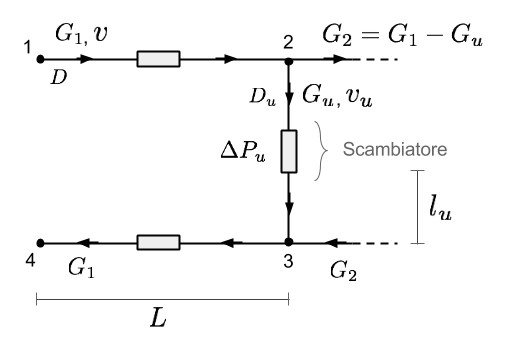
\includegraphics[width=0.70\textwidth]{figure/perdite_carico} % Include the image placeholder.png
\caption{Schema di rappresentativo delle perdite di carico di una porzione della rete di distribuzione}
\label{fig:perdite_carico}

\end{figure}

Dal punto 1 al punto 2 vi è la condotta della rete principale con diametro $D$ che trasporta l'acqua calda mentre da 3 a 4 è la condotta, sempre della rete principale con diametro uguale a quello della condotta da 1 a 2 che trasporta l'acqua raffreddata in ritorno alla centrale di scambio. Entrambe le due condotte sono di lunghezza $L$ identica, in quanto negli impianti le condotte sono sempre poste l'una affianco all'altra. L'acqua scorre a velocità $v$.

Il punto 2 è il punto in cui avviene il prelievo dalla rete principale per portare l'acqua calda all'utenza. Da 2 a 3 abbiamo quindi la condotta che porta l'acqua all'utenza e una che dall'utenza riporta l'acqua alla condotta di ritorno dell'acqua raffreddata con velocità $v_u$. La lunghezza totale è $2 \cdot l_u$ ed il diametro è $D_u$.

Ad ogni condotta può essere associata una certa resistenza che  indica quanto questa si oppone al flusso dell'acqua. Da 1 a 2 oltre alle perdita di carico dovute alle tubazioni vi è anche la perdita di carico che offre lo scambiatore di calore:
\begin{equation}
\Delta P_s = K \ G^2_u
\end{equation}
con K costante che dipende dal tipo di scambiatore.

Le equazioni che descrivono le perdite di carico del sistema sono:

\begin{equation}
\begin{cases}
\Delta P_{12} = \dfrac{\lambda v^2}{2 g D} L = \Delta P_{34} \\
\\
\Delta P_{23} = \dfrac{\lambda v_u^2}{ g D_u} l_u + \Delta P_s
\end{cases}
\end{equation}

Le precedenti equazioni sono usate per ricavare le portate in arrivo alle utenze $G_u$, che rappresentano le variabili incognite d'interesse del sistema descritto. Le portate $G_u$ dipendono principalmente dalla differenza di pressione $\Delta P_{23}$ infatti se questa non è sufficientemente grande non sarà garantito il corretto funzionamento dello scambiatore.

Dal momento che si tratta di un modello fortemente non lineare, si procede all'analisi della rete in modo iterativo. Partendo da dei valori di portata e prevalenza emessi dalla pompa ci ricaviamo la portata $G_u$ della prima utenza incontrata e la portata $G_2$ che andrà ad alimentare tutte le utenze restanti. A questo punto possiamo continuare l'analisi della rete spostandoci all'utenza successiva, ripetendo le operazioni fatte precedentemente, considerando però come portata della condotta principale $G_1$ la portata $G_2$ e così via fino a quando tutte le utenze non sono state analizzate.

Nel caso in cui lo scambiatore d'utenza disponga di una regolazione della portata, allora tale portata, non dipenderà più direttamente dalla differenza di pressione tra i punti 2 e 3, ma sarà determinata dal grado di laminazione della valvola dello scambiatore. 

\section{Perdite di calore nella rete}
Per perdita di calore si intende un trasferimento di 
energia termica tra due sistemi, che è causato da una differenza di temperatura tra i due sistemi in questione. Il calore ceduto da un sistema, a temperatura maggiore, viene acquistato dal secondo sistema, in accordo con la legge di conservazione dell'energia. 
Le perdite di calore in una rete di teleriscaldamento sono proporzionali alla differenza di temperatura del terreno e dell'acqua che circola nelle condotte. Le tubazioni a cui facciamo riferimento sono composte da tubi in acciaio rivestiti da una schiuma isolante poliuretanica, interrati a qualche decina di centimetri.
Le perdite sono quantificate secondo le indicazioni delle norme B.S. (British Standard), assumendo per il coefficiente di conducibilità della schiuma il valore indicato dalle norme CEN EN253 ed utilizzando la formula:

\begin{equation}
\dot{Q}_{disp} = \dfrac{4 \varphi (T_M - T_S)}{\dfrac{1}{\lambda_{PU}} \cdot ln \left(  \dfrac{D - 2t}{d}\right)  + \dfrac{1}{\lambda_S} \cdot ln \left(  \dfrac{2H_S + D}{D}\right) }
\end{equation}

\begin{itemize}
\item $\varphi = \left[ 180 - arctan  D /( D + A_S)  \right] \cdot \pi/180 $  
\item $T_S =$ temperatura del suolo circostante i tubi
\item $T_M =$ media delle temperature di mandata e ritorno del fluido
\item $H_S =$ Altezza del terreno sopra i tubi
\item $A_S =$ spazio tra i tubi in PEAD (polietilene ad alta densità)
\item $d =$ diametro esterno del tubo in acciaio
\item $D =$ diametro esterno del tubo in PEAD
\item $t =$ spessore del tubo in PEAD
\item $Q_{disp} =$ Perdita di calore totale per mandata e ritorno per unità di lunghezza
\item $\lambda_S =$ coefficiente di conduzione termica del suolo
\item $\lambda_{PU} =$ coefficiente di conduzione termica del poliuretano
\end{itemize}

\section{Pompe di circolazione}
Nei sistemi di teleriscaldamento visionati nell'elaborato la circolazione dell'acqua nella rete è resa possibile grazie a delle pompe centrifughe. Queste pompe sono essenzialmente costituite da una girante a palette che gira in una camera a forma di chiocciola [figura \ref{fig:pompa_centrifuga}], comunicante con la tubazione di aspirazione al centro e con la tubazione di mandata alla periferia.

\begin{figure}[h]
\centering
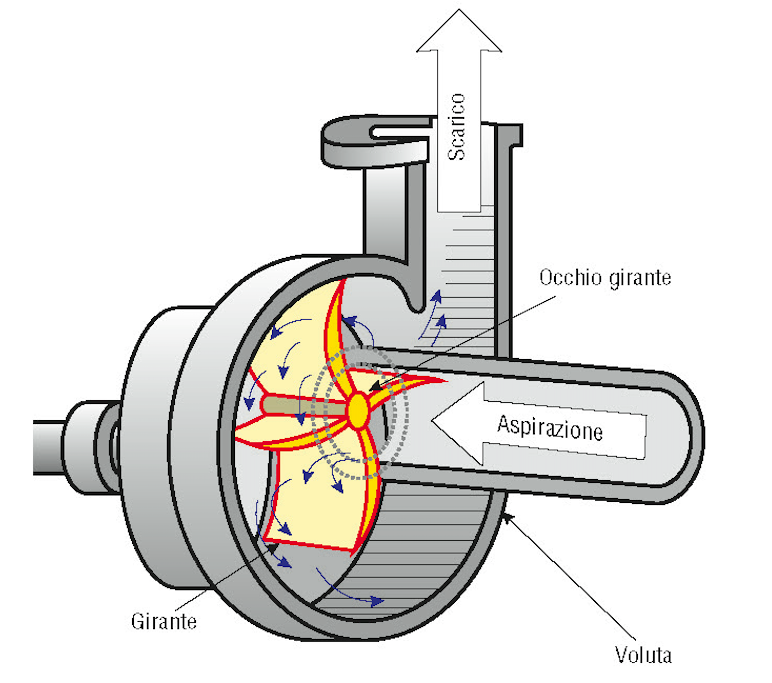
\includegraphics[width=0.65\textwidth]{figure/pompa_centrifuga} 
\caption{Pompa centrifuga con diffusore a palette}
\label{fig:pompa_centrifuga}
\end{figure}

Durante il funzionamento, le palette della girante trascinano in rotazione il liquido e la carcassa lo convoglia verso la tubazione di mandata.
Si determina così una depressione al centro, che richiama altro liquido dalla tubazione di aspirazione, e una spinta in periferia, verso il tubo di mandata.
L'energia acquisita dal liquido attraverso la pompa, cioè la prevalenza manometrica, è in questo caso direttamente proporzionale al quadrato della velocità periferica della girante.
La sezione della camera cresce gradatamente, dall'origine allo sbocco, di pari passo con l'aumentare del liquido che esce uniformemente dalle palette della girante.
La pompa per poter sollevare il fluido deve
essere adescata, cioè sia il condotto di
aspirazione, sia il corpo della pompa devono essere sempre pieni di liquido. Ciò si realizza disponendo all'inizio del condotto di aspirazione una valvola di fondo (o di non ritorno), che permette il passaggio del liquido solo in una direzione e precisamente dal serbatoio alla condotta di aspirazione.
Le pompe centrifughe hanno in genere un rendimento sensibilmente inferiore a quello delle pompe alternativa, principalmente per effetto delle maggiori perdite volumetriche. Sono però notevolmente le più diffuse, per la semplicità di funzionamento e costruttiva e perché possono essere collegate direttamente con i motori elettrici ed endotermici; inoltre non avendo valvole, possono funzionare bene anche con liquidi fangosi.
\subsection{Curve caratteristiche}
La portata e la prevalenza delle pompe centrifughe variano in funzione del numero di giri, inoltre, con il variare della portata varia anche la prevalenza e viceversa. Riportando, in un sistema di assi cartesiani, in ascissa i valori della porta e in ordinata i corrispondenti valori della prevalenza, si ottiene la curva caratteristica della pompa per il numero di giri considerato [figura \ref{fig:curve_car}].

\begin{figure}[!ht]
\centering
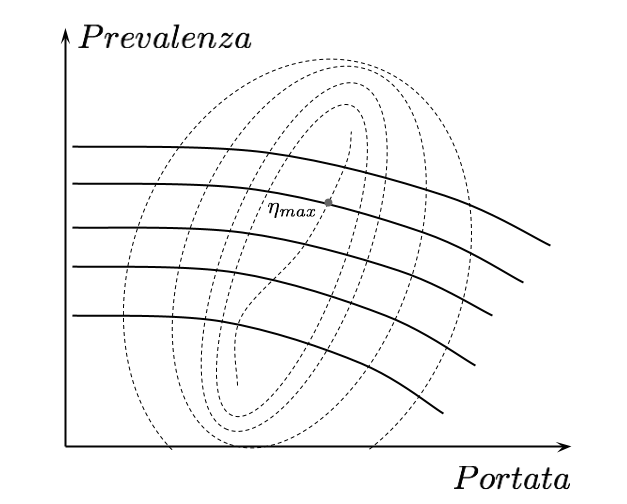
\includegraphics[width=0.65\textwidth]{figure/curve_car} 
\caption{Curve caratteristiche di una pompa centrifuga al variare del numero di giri (linea continua) e curve di rendimento collinari (linea tratteggiata)}
\label{fig:curve_car}
\end{figure}

L'andamento delle curve caratteristiche si può determinare sperimentalmente.
Per questo, sul banco di prova e con la pompa al regime voluto, si varia la portata, agendo
su una valvola di mandata, e per ogni valore della portata si misura il valore della
prevalenza mediante due manometri, uno sulla mandata e uno sull'aspirazione.
Il rendimento della pompa per il regime considerato è massimo solo in un determinato
punto della curva, esiste cioè una sola coppia dei valori di portata e prevalenza per i quali si ottiene
un rendimento idraulico massimo.
Congiungendo tutti i punti nei quali il rendimento ha lo stesso valore, si ottengono delle curve chiuse e concentriche, dette curve di uguale rendimento, o di isorendimento; la linea che unisce i punti di massimo rendimento ($\eta_{max}$) risulta però aperta, perché non esistono in una curva due punti di massimo rendimento.

\subsection{Legge di affinità}
Per le pompe centrifughe esiste una legge che mette in relazione portata, prevalenza e potenza con il numero di giri $n$.
La portata $G$ di una pompa centrifuga varia proporzionalmente al numero di giri; la prevalenza $H_m$ varia proporzionalmente al quadrato del numero di giri; la potenza utile $P$, proporzionale al prodotto della portata per la prevalenza, varia proporzionalmente al cubo del numero di giri:
\begin{equation}
\frac{Q_1}{Q_2}=\frac{n_1}{n_2} \quad \qquad  \frac{H_{m1}}{H_{m2}}=\left( \frac{n_1}{n_2}\right)^2 \quad \qquad  \frac{P_1}{P_2}=\left( \frac{n_1}{n_2}\right)^3
\label{eq:affinita}
\end{equation}
Queste tre espressioni esprimono la legge d'affinità la quale permette di tracciare la curva caratteristica di una pompa ad un regime di rotazione $n_2$ quando è nota la curva relativa ad un regime di rotazione $n_1$, non molto dissimile da $n_2$.

\begin{figure}[!ht]
\centering
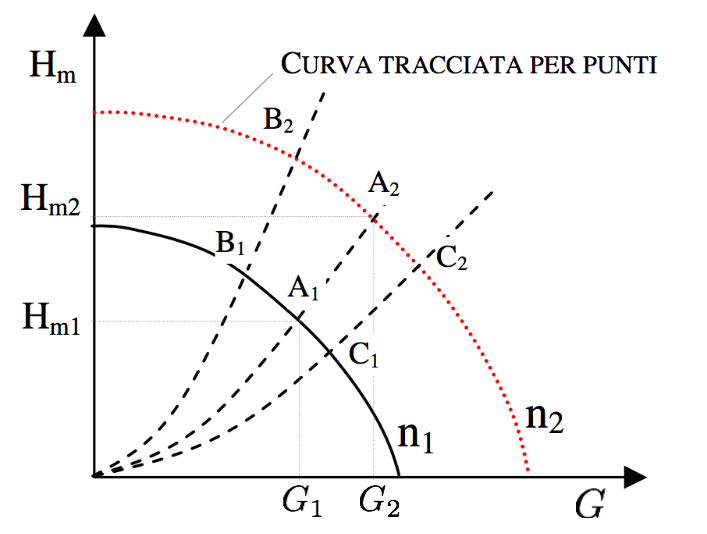
\includegraphics[width=0.65\textwidth]{figure/affinita} 
\caption{Utilizzo della legge di affinità per ricavare da una curva caratteristica nota a regime di rotazione $n_1$ un'altra curva caratteristica avente regime di rotazione $n_2$}
\label{fig:affinita}
\end{figure}

Facendo riferimento alla figura \ref{fig:affinita}, noti per il punto $A_1$ i valori di $G_1$ e $H_{m1}$, si possono determinare:

\begin{center}
$G_2 = \dfrac{n_2}{n_1} \ G_1 \qquad e \qquad H_{m2} = \left( \dfrac{n_2}{n_1}\right)^2  H_{m1}$
\end{center}

che individuano il punto $A_2$. Procedendo in modo analogo per i punti $B_1$, $C_1$ si determinano i corrispondenti punti $B_2$, $C_2$.La curva ottenuta unendo tutti questi punti rappresenta la caratteristica della pompa al regime di rotazione $n_2$.

I punti $A_1$ e $A_2$, $B_1$ e $B_2$, $C_1$ e $C_2$, appartengono a una parabola avente il vertice nell'origine degli assi, infatti dalla legge di affinità:
\begin{center}
$\dfrac{H_{m1}}{H_{m2}}=\left(\dfrac{n_1}{n_2} \right)^2 = \left(\dfrac{G_1}{G_2} \right)^2  \qquad$ ovvero   $\qquad \dfrac{H_{m1}}{G_1^2}=\dfrac{H_{m2}}{G_2^2}$ 
\end{center}
In generale quindi $H_m = K \ G^2$ che corrisponde all'equazione di una parabola passante per l'origine che descrive la resistenza che oppone il circuito alimentato dalla pompa.

La legge di affinità implica che il rendimento della pompa resti invariato alle due velocità. Quindi, due punti appartenenti ala stessa parabola che descrive la caratteristica del circuito risultano avere lo stesso rendimento. In realtà, ciò non è completamente corretto.


\subsection{Potenza assorbita da una pompa}
La pompa, per sollevare una portata d'acqua $G$ fornendole una prevalenza totale $H_m$ compie un lavoro di sollevamento che richiede una potenza $P_u$ (misurata in watt/ora), cioè un'energia, fornitale attraverso un motore, definita dalla seguente espressione:
\begin{equation}
P_u = \rho \ g \ Q \ H_m
\end{equation}
con $\rho$ uguale alla densità del fluido e $g$ l'accelerazione gravitazionale.
La potenza così espressa è la potenza utile, cioè quella strettamente necessaria per sollevare la portata d'acqua $Q$ all'altezza $H_m$. A causa delle inevitabili perdite d'energia la potenza utilizzata, cioè quella realmente necessaria per far funzionare la pompa, è maggiore e viene definita potenza assorbita $P_a$:
\begin{equation}
P_a = \dfrac{\rho \ g \ Q \ H_m}{\eta}
\end{equation}
Il rapporto fra la potenza utile e quella assorbita è definito rendimento ($\eta$). Il rendimento è sempre inferiore all'unità perché in qualsiasi macchina operatrice la potenza utile è sempre minore di quella assorbita. 

\section{Controllo PID}
Il controllo Proporzionale-Integrale-Derivativo, comunemente abbreviato come PID, è un sistema in retroazione negativa ampiamente impiegato nei sistemi di controllo. È il sistema di controllo in retroazione di gran lunga più comune nell'industria, in particolare nella versione PI (senza azione derivativa). Grazie a un input che determina il valore attuale, è in grado di reagire a un eventuale errore positivo o negativo tendendo verso il valore zero. La reazione all'errore può essere regolata e ciò rende questo sistema molto versatile.

Il controllore acquisisce in ingresso un valore da un processo, e lo confronta con un valore di riferimento. La differenza, il cosiddetto segnale di errore, viene quindi usata per determinare il valore della variabile di uscita del controllore, che è la variabile manipolabile del processo.

Il PID regola l'uscita in base a:
\begin{itemize}
\item il valore del segnale di errore (azione proporzionale);
\item i valori passati del segnale di errore (azione integrale);
\item quanto velocemente il segnale di errore varia (azione derivativa).
\end{itemize}

Le tre azioni di un PID vengono calcolate separatamente e semplicemente sommate algebricamente:
\begin{equation}
u=u_P + u_I + u_D 
\end{equation}

L'azione proporzionale è ottenuta moltiplicando il segnale d'errore $e$ con un'opportuna costante $K_P$:
\begin{equation}
u_P = K_P \ e
\end{equation}

L'azione integrale è proporzionale all'integrale nel tempo del segnale di errore $e$, moltiplicato per la costante $K_I$:
\begin{equation}
u_I = K_I \int e(t) dt
\end{equation}
Questa definizione dell'azione integrale fa sì che il controllore abbia memoria dei valori passati del segnale d'errore; in particolare, il valore dell'azione integrale non è necessariamente nullo se è nullo il segnale d'errore. Questa proprietà dà al PID la capacità di portare il processo esattamente al punto di riferimento richiesto, dove la sola azione proporzionale risulterebbe nulla. La presenza dell'integratore può comportare anche il fenomeno del windup.

Per migliorare le prestazioni del controllore si può aggiungere l'azione derivativa:
\begin{equation}
u_D = K_d \ \dfrac{de}{dt} 
\end{equation}
L'idea è compensare rapidamente le variazioni del segnale di errore: se vediamo che $e$ sta aumentando, l'azione derivativa cerca di compensare questa deviazione in ragione della sua velocità di cambiamento, senza aspettare che l'errore diventi significativo (azione proporzionale) o che persista per un certo tempo (azione integrale). \\

Questo particolare controllore verrà in seguito utilizzato per regolare la portata in ingresso ad uno scambiatore agendo su una valvola di laminazione definendo in ogni istante quale dovrà essere la temperatura di mandata ai radiatori.

\chapter{Risultati della simulazione}
L'ottimizzazione e il controllo delle reti di teleriscaldamento è di grande interesse per industria energetica a causa dei vantaggi tecnici, economici e ambientali che potrebbero essere guadagnati da una gestione adeguata. Tuttavia, i modelli di questi sistemi complessi, sono fortemente non lineari  e soffrono di incertezze rilevanti. Nel nostro lavoro abbiamo implementato una simulatore di una rete di teleriscaldamento per analizzare e confrontare diverse strategie di controllo che riducano al minimo i costi di gestione di un impianto.
Il punto di partenza per ottimizzare l'intero impianto consiste nell'incrementare l'efficienza delle utenze, abbattendo al massimo la temperatura dell'acqua di ritorno dagli scambiatori 
e riducendo gli sprechi anche in situazioni di cattiva gestione 
della regolazione della temperatura all'interno delle abitazioni.

La calibrazione dei risultati ottenuti con le simulazioni è stata eseguita confrontando questi con dati misurati sul campo.
In simulazione è stato preso in esame un piccolo impianto di teleriscaldamento composto da undici utenze. Nonostante le ridotte dimensioni, il suo studio risulta di particolare interesse in quanto l'impianto a causa di un cattivo sistema di regolazioni fa si che i costi di gestione siano quasi sempre vicini al massimo stagionale (consumi che si hanno nel periodo più freddo dell'anno). Inoltre, le ridotte dimensioni ci hanno permesso di facilitarci nella simulazione e nella raccolta dei dati necessari alla calibrazione del sistema.  

\section{Caratteristiche di un'utenza termica}

\textit{spiegare come il calore richiesto dipende dalla temperatura esterna e inserire immagine e dire che maggiore potenza è fornita (temp in mandata più alta) si avrà un ritorno più alto}

\begin{figure}[!ht]
\centering
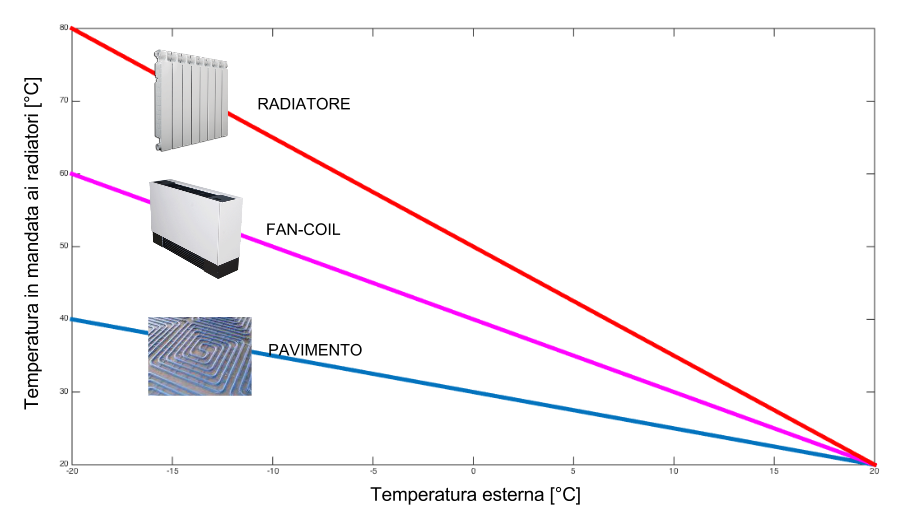
\includegraphics[width=0.85\textwidth]{figure/elem_scaldanti} 
\caption{Temperature di funzionamento di vari tipi di elementi scaldanti al variare della temperatura esterna}
\label{fig:elem_scaldanti}
\end{figure}

\begin{figure}[!ht]
\centering
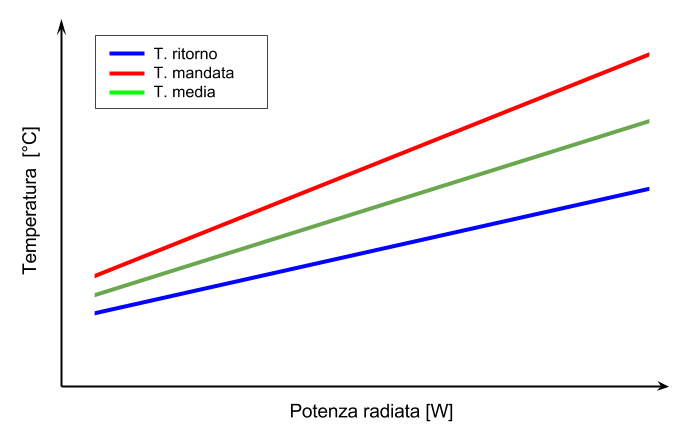
\includegraphics[width=0.85\textwidth]{figure/pot_radiatore} 
\caption{}
\label{fig:pot_radiatore}
\end{figure}

\section{Funzionamento e importanza dell'utilizzo di centraline d'utenza}

Le centralina d'utenza rappresenta un elemento dell'impianto di teleriscaldamento posizionato nell'abitazione. La centralina è composta da uno oppure due scambiatori: il primo nel caso in cui si utilizzi il teleriscaldamento soltanto per scaldare gli ambienti mentre il secondo nel caso si voglia produrre anche acqua calda ad uso sanitario. Nella condotta che porta l'acqua calda alla sottostazione è posizionata un'elettrovalvola di laminazione  che permette la regolazione del flusso di acqua in ingresso allo scambiatore. Il grado di chiusura della valvola è determinato da una centralina in base al criterio di controllo scelto. Le regolazioni che possono essere implementate sono le seguenti e verranno approfondite in seguito:

\begin{itemize}
\item regolazione a punto fisso;
\item termoregolazione climatica;
\item regolazione climatica evoluta PI.
\end{itemize}  

Lo schema in figura \ref{fig:} rappresenta una centralina d'utenza adibita alla produzione combinata del riscaldamento e dell'acqua igenico sanitaria.

\begin{figure}[!ht]
\centering
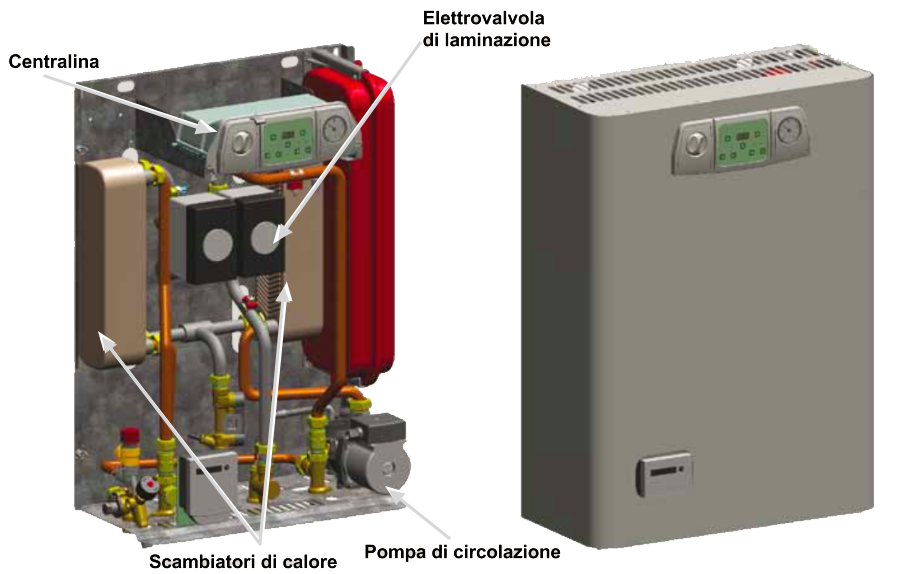
\includegraphics[width=0.85\textwidth]{figure/centralina} 
\caption{Schema di una sottostazione d'utenza con centralina}
\label{fig:centralina}
\end{figure}

% spiegare funzionamento.

Le sottostazioni d'utenza con centralina, devono permettere anche un'analisi di predittiva sullo stato di funzionamento degli scambiatori con segnalazione di anomalie che portano ad interventi programmati invece che in accidentale, il tutto per avere un sistema sempre funzionante al massimo dell'efficienza.

Di notevole importanza è che le centraline delle utenze più svantaggiate (ovvero quelle che hanno la portata più bassa nel sistema) comunichino informazioni alla stazione di pompaggio per ottimizzare la portata delle pompe per garantire a tutte le utenze il necessario flusso di acqua per il proprio fabbisogno. 

% spiegare meglio (più approfonditamente dicendo che ora i sensori sono nella centrale di scambio ed eventuali portate non sufficienti sono comunicate dagli utenti perchè i radiatori sono freddi)


Riassumendo, i sistemi di regolazione delle centraline d'utenza devono:
\begin{itemize}
\item controllare che i flussi nello scambiatore siano quelli ottimali, limitando la portata secondo la regolazione più opportuna;
\item controllare che nello scambiatore vi sia il massimo abbattimento di temperatura possibile, evitando che circoli inutilmente acqua calda;
\item aiutare a fare efficienza al cliente finale, utilizzando la termoregolazione climatica che definisce il carico termico massimo da fornire all'utenza in base alla temperatura esterna;
\item permettere al gestore di avere utili indicazione per interventi manutentivi come nel caso di intasamento degli scambiatori oppure una bassa differenza di pressione ai capi
\item le centraline dei punti più svantaggiati devono fornire informazioni per ottimizzare la portata delle pompe principali di regolazione.
\end{itemize}

Esistono centraline nel mercato che però non realizzano tutti questi obiettivi.

\section{Soluzioni per aumentare l'efficienza delle utenze diminuendo la temperatura dell'acqua di ritorno}
Nonostante i problemi che comportano le reti di distribuzione senza regolazioni di portata in arrivo alle utenze, circa duemila sono gli scambiatori gestiti da GES che ne sono privi.
Dettò ciò andremo a studiare alcuni tipi di regolazioni che aumentino l'efficienza delle abitazioni. 
Come base di paragone per tutte le simulazioni future verrà preso in considerazione uno scambiatore senza limitatore di portata: tutto il flusso di acqua in arrivo allo scambiatore verrà utilizzato per fornire calore all'acqua del circuito dell'utenza. 


%La regolazione dell'impianto può seguire due principi: a punto fisso, cioè con temperatura di mandata fissata indipendentemente dalle condizioni esterne; climatica, cioè con adeguamento continuo alla situazione di temperatura esterna. La climatica del futuro ormai prossimo, sarà una regolazione evoluta, che ottimizza i consumi in funzione del comfort, tutto questo sarà possibile grazie all'algoritmo PI.

\subsection{Termoregolazione a punto fisso}
Si tratta del sistema di regolazione più semplice. La regolazione a punto fisso garantisce all'impianto una temperatura del fluido di mandata costante. 

Il valore viene impostato manualmente attraverso una valvola termostatica che regola la portata in ingresso allo scambiatore.  

Il limite maggiore è la necessità, da parte dell'utilizzatore, di dover regolare l'impianto ogni volta che variano le condizioni esterne. Per ridurre questa esigenza si è diffusa la consuetudine di tarare la valvola termostatica sulla temperatura di progetto, uguale alla massima temperatura necessaria nel giorno più freddo dell'anno. In questo modo però nei giorni meno freddi si avrà un surplus di energia che riduce l'efficienza dell'abitazione.

Il termostato confronta la temperatura impostata dall'utilizzatore con quella presente e, se la temperatura in ambiente supera quella impostata, toglie corrente alla pompa di circolazione e chiude la valvola di laminazione, interrompendo il flusso di acqua nello scambiatore d'utenza. 

Quando la temperatura in ambiente è scesa fino ad essere inferiore a quella richiesta, il termostato comanda la riapertura, in modo da garantire nuovamente la temperatura ideale.

\begin{figure}[!ht]
\centering
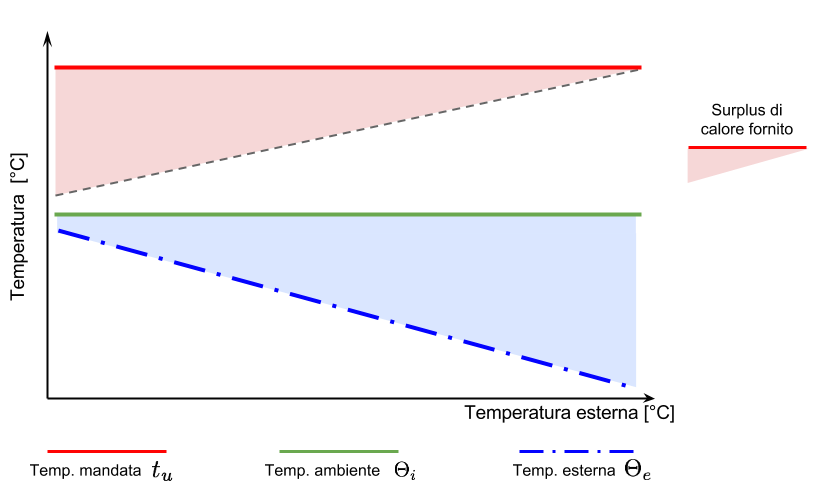
\includegraphics[width=0.85\textwidth]{figure/surplus} 
\caption{Nella regolazione a punto fisso l'acqua circola alla temperatura corrispondente al valore necessario per il giorno più freddo dell'inverno. Nel grafico sono mostrati i surplus di energia in funzione della temperatura esterna}
\label{fig:surplus}
\end{figure}

\subsection{Termoregolazione climatica}
Poiché il calore necessario per mantenere le condizioni di comfort in ambiente è legato alle dispersioni dell'edificio ed alla temperatura esterna, il fabbisogno termico aumenta all'aumentare delle dispersioni dell'edificio e al diminuire della temperatura esterna. Le regolazioni di tipo climatico permettono di selezionare una curva climatica all'interno di una famiglia di curve, in modo da adeguare la regolazione allo specifico edificio. 

Fissata la curva climatica, la temperatura di mandata all'impianto viene regolata in modo automatico in funzione della temperatura esterna, adeguando l'apporto di calore al fabbisogno termico dell'edificio, per garantire sempre le migliori prestazioni in termini di comfort. 

\begin{figure}[!ht]
\centering
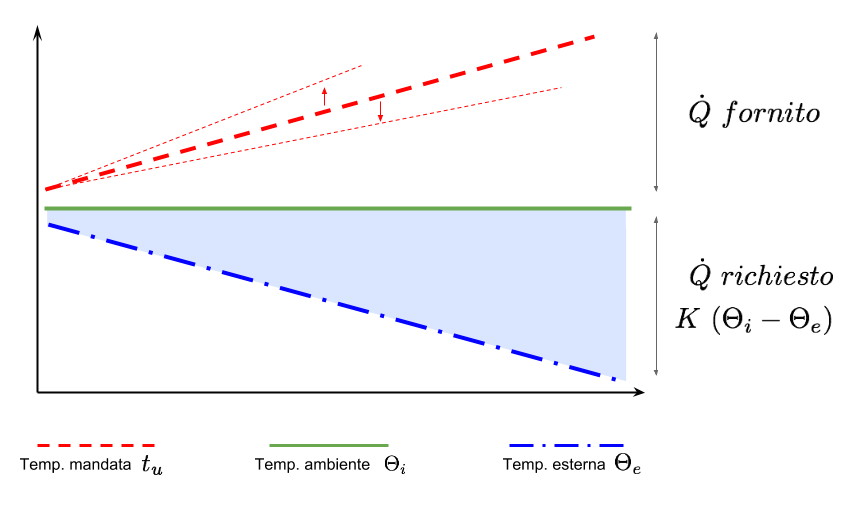
\includegraphics[width=0.85\textwidth]{figure/climatica} 
\caption{La regolazione climatica regola la temperatura di mandata in funzione del calore necessario (funzione della temperatura esterna) e la pendenza della $t_u$ mandata dipende dal fabbisogno termico dell'edificio}
\label{fig:surplus}
\end{figure}

Per ottenere questi risultati si utilizza una centralina elettronica digitale, a cui sono collegate due sonde di temperatura: una di mandata all'impianto e una esterna. 

La centralina elabora il segnale della sonda esterna e, in base al codice climatico più adatto per quel tipo di edificio, determina il valore ideale della temperatura di mandata, lo confronta con il valore reale misurato dalla sonda di mandata e, se necessario, agisce sull'elettrovalvola posizionata nella condotta in ingresso allo scambiatore per regolare la portata di acqua calda.

La curva climatica o curva di riscaldamento è il rapporto tra la temperatura esterna e la temperatura di mandata ai corpi scaldanti. Per un corretto dimensionamento di tale curva si necessita la conoscenza di due parametri:
\begin{itemize}
\item Temperatura esterna minima di progetto
\item Temperatura massima di mandata all'impianto di riscaldamento
\end{itemize}
Conosciuti questi valori si andranno a congiungere le due rette corrispondenti sul grafico, trovando in questo modo la curva da inserire.

\subsection{La regolazione climatica evoluta PI}
Una regolazione climatica evoluta è in grado di gestire in modo ottimale il comfort indoor per quanto riguarda la climatizzazione invernale.

Ogni volta che un dispositivo deve mantenere costante un determinato valore, ad esempio una velocità, una temperatura, un livello, una rotta ecc. serve un regolatore. Ci serve qualcosa che corregga eventuali ed inevitabili errori rispetto al valore di consegna.
 
Se impostiamo una temperatura all'interno di un ambiente, il regolatore deve poter correggere errori dovuti alle continue variazioni ambientali sia interne che esterne, come la variazione delle dispersioni termiche verso l'esterno, la variazione del contributo dovuto all'irraggiamento durante le diverse ore del giorno, le dispersioni oppure gli apporti interni dovuti alla presenza di persone e all'accensione di apparecchiature elettriche.

Questa gestione ottimizzata  del comfort è possibile grazie ad un sistema di regolazione proporzionale integrale, chiamato più semplicemente PI, che rappresenta il sistema più efficiente per il controllo della temperatura dell'ambiente. L'azione derivativa è stata tralasciata perché renderebbe il controllore troppo sensibile: un PID con azione derivativa, per esempio, subirebbe una brusca variazione nel momento in cui il riferimento venisse cambiato quasi istantaneamente da un valore a un altro, risultando in una derivata dell'errore tendente a infinito, o comunque molto elevata. Ciò sconsiglia l'applicazione dell'azione derivativa in tutti i casi in cui l'attuatore fisico non deve essere sottoposto a sforzi eccessivi.

Il sistema di controllo agisce direttamente sull'elettrovalvola di laminazione posizionata in ingresso allo scambiatore. In base al valore della differenza tra temperatura desiderata e temperatura ambiente il controllore decide la migliore temperatura in mandata ai radiatori. Il PI agisce sulla regolazione in base a 2 azioni:
\begin{itemize}
\item Azione proporzionale: controllo sul valore all'istante della temperatura ambiente
\item  Azione integrale: controllo basato sui valori passati della temperatura ambiente
\end{itemize}
Uno schema di funzionamento del controllo PI è mostrato in figura \ref{fig:PI}.

\begin{figure}[!ht]
\centering
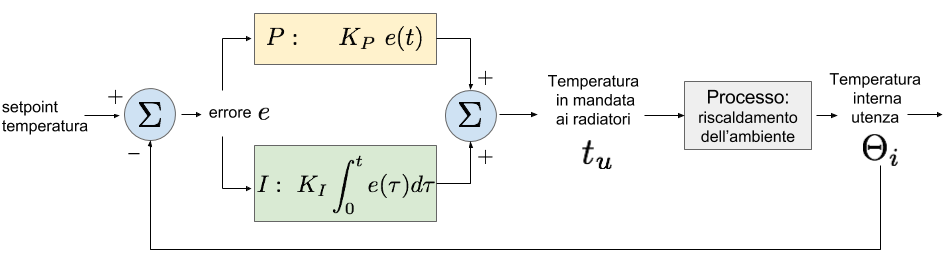
\includegraphics[width=1.05\textwidth]{figure/PI} 
\caption{Schema a blocchi di un controllore PI usato per la termoregolazione di un'utenza}
\label{fig:PI}
\end{figure}
   
L'utente può in ogni caso impostare un valore di temperatura molto elevato nel termostato. Per aiutare l'utilizzatore dell'impianto di riscaldamento a fare ulteriore efficienza, la temperatura dell'acqua in mandata ai radiatori avrà un limite massimo sulla base della temperatura esterna e delle caratteristiche dell'edificio, secondo il concetto di termoregolazione climatica. 
Ovviamente questa temperatura limite dovrà garantire all'abitazione di potersi scaldare fino ad una temperatura di circa $20 ^{\circ}C$.

L'introduzione di questi limiti di saturazione sul controllore potrebbero introdurre effetti di windup.
Supponendo di applicare al sistema di riferimento un errore elevato, l'integratore inizierà ad accrescere il suo valore in uscita per via dell'errore non nullo. Quando il valore in uscita al controllore è tale da saturare il comando di attuazione, l'uscita dell'integratore continuerà a crescere fino a quando l'errore non diventerà nullo.
Il termine integrale può raggiungere valori molto elevati: è quindi richiesto che l'errore presenti segno opposto per un lungo periodo prima che si esca dalla saturazione. 
Questo fenomeno fa sì che il sistema dopo aver raggiunto la condizione di errore nullo, si allontani in direzione opposta, creando un effetto di sovraelongazione dalle caratteristiche non lineari.\\

% soluzione utilizzata o NON utilizzata (spiegare perchè)

La soluzione che utilizza un controllo PI per regolare il calore fornito ai radiatori, elimina le oscillazioni della temperatura interna dell'abitazione e richiede in ogni momento sempre la minima quantità di calore necessario per il comfort richiesto. Le temperature di ritorno dell'acqua alla centrale di scambio, saranno tanto più basse tanto è minore il carico termico richiesto. 

 


\section{Soluzioni per ridurre i consumi di energia di pompaggio}

\subsection{Vantaggi di utilizzare pompe a velocità variabile}
Un numero crescente di aziende si sta accorgendo dell'importanza dell'efficienza energetica e dell'impatto che essa esercita sui costi e sui profitti dell'azienda.
In particolare, il prodotto che più immediatamente e in maniera consistente permette di conseguire dei risparmi energetici è l'inverter, soprattutto in applicazioni con movimentazione di fluidi, come ad esempio pompe centrifughe. Infatti, per tali applicazioni, è valida una legge fisica, chiamata "legge di affinità" (eq. \ref{eq:affinita}), la quale afferma che la potenza assorbita è proporzionale al cubo della velocità di rotazione del motore. Da tale condizione è facile capire come, dimezzando la velocità del motore, la potenza impiegata sarà di un ottavo della potenza a regime. 
Applicando un inverter, a ogni variazione di velocità viene generata una nuova curva caratteristica, ciò significa che, variando la velocità di rotazione della pompa, si ottiene una nuova macchina con caratteristiche di funzionamento analoghe alla precedente, ma nettamente diversa. Quando si raggiungono basse velocità di rotazione si verifica un calo sensibile del rendimento. Variando il numero di giri della pompa variano sensibilmente gli assorbimenti della potenza, come evidenziato anche dalle relazioni di proporzionalità. Gli effetti benefici della variazione di velocità sono facilmente comprensibili mettendo in relazione la tecnica di controllo “con valvola di laminazione” e con l’utilizzo di inverter. 

La valvola di laminazione effettua una riduzione della sezione della conduttura attraversata dal fluido, quindi in tale condizione se si desidera ridurre la portata della pompa centrifuga a portata inferiore, si sposta il punto di funzionamento, come risulta evidente dalla figura \ref{fig:strozzatura}.

\begin{figure}[!ht]
\centering
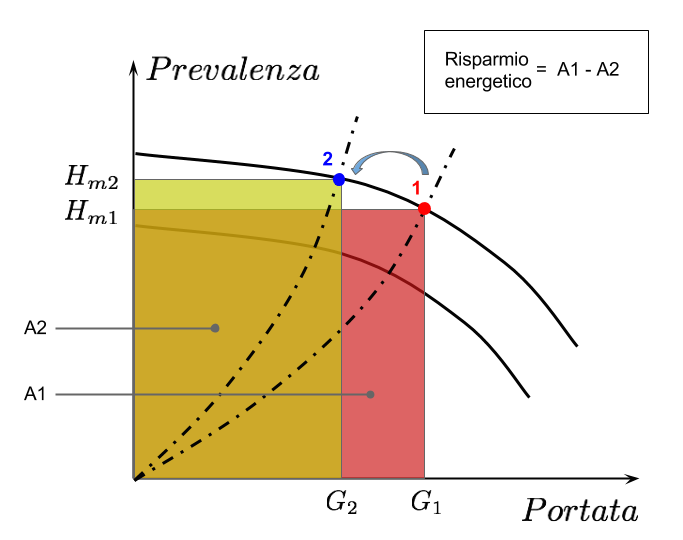
\includegraphics[width=0.75\textwidth]{figure/strozzatura} 
\caption{Rappresentazione dell'energia salvata riducendo la portata con valvola di laminazione}
\label{fig:strozzatura}
\end{figure}

Il punto di funzionamento della pompa si sposta da $1$ a $2$, imponendo di fatto un maggiore valore di prevalenza dell'impianto. Utilizzando un inverter si riduce il numero di giri della pompa, quindi ci si sposta lungo la curva dell'impianto e non della pompa come è possibile vedere in figura \ref{fig:var_velocita}. 

\begin{figure}[!ht]
\centering
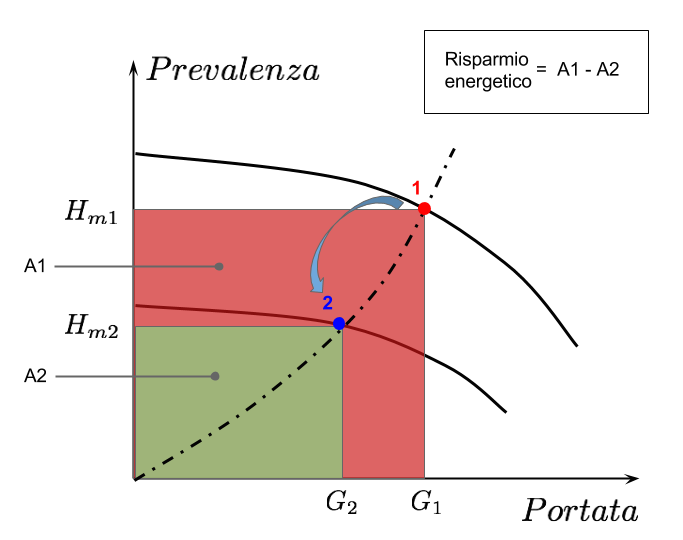
\includegraphics[width=0.75\textwidth]{figure/var_velocita} 
\caption{Rappresentazione dell'energia salvata riducendo la portata variando la velocità delle pompe}
\label{fig:var_velocita}
\end{figure}

Dal punto di vista energetico la differenza è sostanziale: l'energia consumata è proporzionale alla differenza tra le due aree $A2$ e $A1$. Con la valvola di strozzatura il vantaggio è minimo, mentre nel secondo caso, grazie all'impiego di un inverter, l'incremento di efficienza energetica è decisamente più importante.


\section{Caratteristiche dell'impianto di Sant'Ippolito}
Il sistema analizzato in simulazione è la rete di teleriscaldamento chiamata S. Ippolito. \`E costituito da una centrale di cambio con scambiatore di calore vapore - acqua. La temperatura dell'acqua in mandata alla rete di distribuzione è regolata da una valvola di laminazione che regola il flusso di vapore in ingresso allo scambiatore. La temperatura desiderata di mandata è decisa arbitrariamente in base alla stagione. Nella centrale di scambio è presente una stazione di pompaggio con pompe a velocità variabile.
Le utenze allacciate ala rete dispongono di un sistema che regola il flusso in ingresso ai radiatori così da mantenere fissa la temperatura in mandata ai radiatori dell'abitazione. Questo tipo di regolazione aiuta ad abbattere la temperatura di ritorno rispetto a dei normali  scambiatori senza regolazioni di portata. La riduzione della temperatura di ritorno dovrebbe aiutare a limitare i consumi di energia di pompaggio, ma un sistema di regolazioni non adeguato rende il tutto invano. Le pompe sono controllate nel seguente modo: si vuole mantenere la temperatura dell'acqua di ritorno alla centrale di scambio ad un certo valore di temperatura prestabilito. Dal momento che è possibile regolare la velocità delle pompe, questa regolazione   risulterebbe efficiente nel caso le utenze avessero duna configurazione con valvole a tre vie come in ... . Nella situazione attuale, invece, quando le utenze richiedono poco calore, le valvole di laminazione si chiudono quasi totalmente facendo passare solo una piccola quantità di acqua nello scambiatore di utenza. L'acqua in circolo a causa della portata ridotta cederà gran parte del suo calore e l'abbattimento di temperatura sarà elevato. La situazione che si può verificare, è quella di avere l'acqua di ritorno a temperatura minore di quella impostata come set point cosicché i sensori ordineranno alle pompe di aumentare la velocità per incrementare la portata  nel circuito ed innalzare la temperatura dell'acqua. Ciò che si verifica è avere le pompe che lavorano quasi sempre al massimo dei giri sopratutto nei periodi con bassa richiesta di calore da parte delle utenze.



\begin{table}[]
\centering
\begin{tabular}{|c|c|c|c|}
\hline
\multicolumn{4}{|c|}{Tipologie di condotte nella rete di distribuzione}                                                                                                                                                   \\ \hline
Nome & \begin{tabular}[c]{@{}c@{}}Diametro\\ interno {[}mm{]}\end{tabular} & \begin{tabular}[c]{@{}c@{}}Diametro \\ esterno {[}mm{]}\end{tabular} & \begin{tabular}[c]{@{}c@{}}Spessore \\ isolante {[}cm{]}\end{tabular} \\ \hline
DN65 & 70,3                                                                & 73,2                                                                 & 2,895                                                                 \\ \hline
DN50 & 54,5                                                                & 57,4                                                                 & 2,935                                                                 \\ \hline
DN40 & 43,1                                                                & 45,7                                                                 & 2,785                                                                 \\ \hline
DN32 & 37,2                                                                & 39,8                                                                 & 3,1                                                                   \\ \hline
d.28 & 24,2                                                                & 28                                                                   & -                                                                     \\ \hline
\end{tabular}
\caption{My caption}
\label{tab:condotte}
\end{table}


\begin{table}[]
\centering
\begin{tabular}{|c|c|c|c|c|c|c|}
\hline
\multicolumn{7}{|c|}{Rete di distribuzione S. Ippolito}                                                                                                                                                       \\ \hline
\multicolumn{1}{|c|}{\multirow{2}{*}{Utenze}} & \multicolumn{2}{c|}{Condotta Primaria}                         & \multicolumn{2}{l|}{Condotta intermedia}          & \multicolumn{2}{c|}{Condotta secondaria} \\ \cline{2-7} 
\multicolumn{1}{|c|}{}                        & Tipo                  & \multicolumn{1}{l|}{Lunghezza {[}m{]}} & \multicolumn{1}{l|}{Tipo} & Lunghezza {[}m{]}     & Tipo         & Lunghezza {[}m{]}         \\ \hline
1                                             & \multirow{2}{*}{DN65} & \multirow{2}{*}{235,6}                 & \multirow{2}{*}{DN32}     & \multirow{2}{*}{12,7} & d.28         & 24,5                      \\ \cline{1-1} \cline{6-7} 
2                                             &                       &                                        &                           &                       & d.28         & 3,5                       \\ \hline
3                                             & DN65                  & 25,8                                   & -                         & -                     & d.28         & 57,6                      \\ \hline
4                                             & DN65                  & 20                                     & -                         & -                     & d.28         & 12,4                      \\ \hline
5                                             & DN65                  & 111                                    & -                         & -                     & d.28         & 33,7                      \\ \hline
6                                             & DN65                  & 1082                                   & -                         & -                     & d.28         & 36                        \\ \hline
7                                             & DN65                  & 65                                     & -                         & -                     & d.28         & 16,5                      \\ \hline
8                                             & \multirow{2}{*}{DN50} & \multirow{2}{*}{168}                   & \multirow{2}{*}{DN32}     & \multirow{2}{*}{70}   & d.28         & 34,5                      \\ \cline{1-1} \cline{6-7} 
9                                             &                       &                                        &                           &                       & d.28         & 40                        \\ \hline
10                                            & DN50                  & 109,8                                  & -                         & -                     & d.28         & 7,3                       \\ \hline
11                                            & DN50                  & 30,3                                   & -                         & -                     & DN40         & 341,2                     \\ \hline
\end{tabular}
\caption{My caption}
\label{tab:rete_ippolito}
\end{table}


\subsection{Simulazione rete senza regolazioni}

\subsection{Simulazione rete con regolazione in mandata}



\chapter{Conclusioni}


\backmatter

%%%%%%%%%%%%%%%
% Appendici
%%%%%%%%%%%%%%%
\appendix
\chapter{Appendice A: Dettagli}
%\input{introapp}
Le appendici possono riportare dettagli che vengono omessi nei
Capitoli. In genere possono contenere dimostrazioni di risultati
presentati, tabelle di dati o documenti di supporto al materiale
esposto nei Capitoli.

Le Appendici possono avere varia lunghezza a seconda del materiale
che si ritiene opportuno presentare.


%%%%%%%%%%%%%%%
% Bibliografia
%%%%%%%%%%%%%%%
%\input{biblio}           % Bibliografia
%


\bibliographystyle{IEEEbib}
%\bibliographystyle{unsrt}
\bibliography{FileBiblio}
\end{document}
\bigotimes
